\documentclass[a4paper, 12pt, openany]{book} %chose the paper size and font size. Openany ensures that all all chapters and similar may begin at any page, not only odd pages. For the introductory pages and appendices we want openany, but for chapter pages in the main content we want chapters to begin only on odd pages (right hand side). The book class ensures that the margins are automatically adjusted such that left hand pages are slightly moved to the left and vice versa at the right, which makes the thesis very readable and good looking when printed in bound book format.
\usepackage[utf8]{inputenc} %to manage special characters
\usepackage[T1]{fontenc} %to manage special characters
\usepackage[Bjarne]{fncychap} %fancy chapter style (many more available, like Sonny or Lenny etc.)
\usepackage{fancyhdr} %to customize the headers
\usepackage[lmargin=1.5in, rmargin=1in, tmargin=1in, bmargin=1in]{geometry} %sets the margins for the pages
\setcounter{tocdepth}{2} %table of contents number depth for subsections (2 = x.x.x)
\setcounter{secnumdepth}{4} %numbering depth for headers for subsections in the text(4 = x.x.x.x)
\usepackage{url} %to include urls
\usepackage{listings} %include this if you want to include code in the thesis
\usepackage{amsmath,amssymb} %mathematical package
\usepackage{siunitx} %includes SI-units
\usepackage[bf]{caption} %makes float captions bold
\usepackage{array, booktabs} %to make better tables
\usepackage{graphicx} %to include graphics
\usepackage{float} %to include floats
\usepackage[export]{adjustbox} %to adjust floats
\usepackage{subfig} %to include subfigures
\usepackage{chngcntr} %will make it possible to change the counter for tables, figures etc. such as below
\counterwithin{figure}{section} %change counter for figures within sections (also possible to choose for each chapter
\counterwithin{table}{section} %change counter for tables within sections
\usepackage{color, xcolor} %edit e.g. text colors

\usepackage[backend = biber,
            style = numeric,
            date = long,     % Long: 24th Mar. 1997 | Short: 24/03/1997
            sorting = none,
            maxcitenames = 3,   % max names to include before et. al.
            ]{biblatex} %customize the look of your citations and bibliography
\addbibresource{bibliography.bib} %declare the bibliography resource
\usepackage{comment} %to be able to comment out sections in the .tex files
\usepackage{afterpage} %to customize page commands such as below
\newcommand\myemptypage{
    \null
    \thispagestyle{empty}
    \addtocounter{page}{-1}
    \newpage
    } %sets new page command to insert an empty page without adding to the page counter or having a page number



\begin{document}
%%%%%%%%%%%%%%%%%%%%%%%%%%%%%%%%%%%%%%%%%%%%%%%%%%%%%%%%
%\begin{comment}
% The title page:
% For NTNU students this page will be generated automatically when submitting your paper, and should not be included in the final file from Latex. Delete or comment out the title page setup. The final report should then start with the first page being the abstract. I have included a title page here so it is possible to see how it may look like, and for those who does not get an automatically generated title page. Of course you will need to change the names and titles etc. to your case.

%the title page should be an odd page (right hand side)

\begin{titlepage}
\newgeometry{left=1.6in, right=2in}
\vspace*{1cm}

\begin{figure}[h]
    
\includegraphics[height=0.32\textwidth]{Figures/logo_polito.jpg}
    \centering
\end{figure}

\vspace*{1.2cm}

\noindent  \textcolor{gray}{\large Davide Aimar} \\
\vspace{0.4cm}

\noindent \textbf{\Large Extraction, indexing and analysis of Ethereum Smart Contracts} \\
\vspace{5.5cm}


\noindent Master's thesis in Computer Engineering \\
Supervisor: Prof.ssa Valentina Gatteschi \\
Co-supervisor: Prof. Mariusz Nowostawski \\
A.A. 2022/2023 \\

\vspace{0.2cm}
\noindent Politecnico di Torino \\

\vspace{0.2cm}
\noindent In collaboration with\\
Norwegian University of Science and Technology

\end{titlepage}
\restoregeometry
\myemptypage %empty page such that the abstract starts at the first right hand side after the title page
%\end{comment}
%%%%%%%%%%%%%%%%%%%%%%%%%%%%%%%%%%%%%%%%%%%%%%%%%%%%%%%%

% The pre-chapters
\chapter*{Abstract} %pre-chapters should not be numbered, hence the "*"
\pagenumbering{roman} %introductory pages should be roman
\setcounter{page}{1}
\addcontentsline{toc}{chapter}{\protect\numberline{}Abstract} %add the chapter to the table of contents, this is not automatically added when creating unnumbered chapters (*). Add it in a chapter style, and keep all chapters on the same numberline indent regardless of number or not on the chapter
Blockchain technology has gained popularity in the last decade. New protocols allow developers to build decentralized applications thanks to the usage of smart contracts. Ethereum is one of the most popular blockchain networks of this kind. Every twelve seconds, a new block is appended to this chain. Each block contains information that describes a market worth billions of dollars. Since Ethereum is a permissionless blockchain, this data is publicly available to anyone, but without proper tools, it is not easy to analyse.

This master's thesis focuses on extracting semantics from raw Ethereum data and making it easily available to users by indexing it with Dgraph, an open-source distributed graph database. 

A review of the state-of-the-art tools showed that relevant work in this field has been done by private companies whose source code and methodology are not available. Many open-source and public projects resulted in being outdated or slow. This poses the risk of centralizing access to blockchain data in the hands of a few companies.

Part of this master's thesis was dedicated to analyzing the semantics that can be extracted from the blockchain and building a data schema around it that is optimized for graph databases. A custom software, called~\textit{eth2dgraph}, was developed to perform the extraction of data. It is an open-source tool written in \textit{Rust} that maps Ethereum data to Dgraph format. It integrates a decompiler to extract and index the ABI of smart contracts. Eth2dgraph was developed with a focus on performance. This was done to scale the extraction process to the history of the Ethereum blockchain. At the end of the thesis, the data indexed in Dgraph has been analyzed to show the current state of the Ethereum blockchain.

This work provides a novel solution to the problem of blockchain data analysis. The open-source nature of the project allows other developers to build on top of it. Performing the actual extraction and indexing came close to hitting the limit of what can be done on a single machine. This highlights the fact that, in the future, distributed approaches will be the only possible way of handling the increasing amount of data that comes from the Ethereum blockchain. This is already evident with layer 2 protocols, which are generating data at a faster pace than Ethereum.

 %insert the chapter text from the files

\chapter*{Preface}
\addcontentsline{toc}{chapter}{\protect\numberline{}Preface} 

Write the preface of your thesis here. \\

\noindent You may include acknowledgements and thanks as part of your preface on this page, or you may add it as a new chapter after the preface.

\tableofcontents
\addcontentsline{toc}{chapter}{\protect\numberline{}Contents}

%add to table of contents list of figures and tables, and insert list of figures and tables
\addcontentsline{toc}{chapter}{\protect\numberline{}\listfigurename}
\listoffigures
\addcontentsline{toc}{chapter}{\protect\numberline{}\listtablename}
\listoftables


\chapter*{Abbreviations}
\addcontentsline{toc}{chapter}{\protect\numberline{}Abbreviations}
% Put in your abbreviations here

List of all abbreviations in alphabetic order:

\begin{itemize}
    \item \textbf{ABI} Application Binary Interface
    \item \textbf{CHF} Cryptographic hash function
    \item \textbf{dApp} Decentralized Application
    \item \textbf{DQL} Dgraph Query Language
    \item \textbf{EOA} Externally Owned Account
    \item \textbf{EVM} Ethereum Virtual Machine
    \item \textbf{SC} Smart Contract
    \item \textbf{RPC} Remote Procedure Call
    \item \textbf{NFT} Non Fungible Token
\end{itemize}
\newpage
\myemptypage
%add an empty non-counted page by the command below in order to get the first chapter on the left hand side, if needed (check your page number so that the first chapter is on an odd page)


%%%%%%%%%%%%%%%%%%%%%%%%%%%%%%%%%%%%%%%%%%%%%%%%%%%%%%%%
%Customize the layout of the main content of your thesis

\pagestyle{fancy} %set customized page style for header
\fancyhf{} %clear header and footer fields
\renewcommand{\headrulewidth}{0pt} %set to no rule
\fancyhead[LE, RO]{\thepage} %set the page number at left for even, right for odd pages
\fancyhead[RE, LO]{\leftmark} %set the chapter name at right for even, left for odd pages
%is is possible to design the header with the chapter as you wish, e.q. only the chapter or only the name, all lowercase instead etc.
%you could also design the footer if you wish, for example:
%\fancyfoot[LE, RO]{\thepage}
\setlength{\headheight}{14.49998pt} %set the header height


%%%%%%%%%%%%%%%%%%%%%%%%%%%%%%%%%%%%%%%%%%%%%%%%%%%%%%%%
%main content 

\pagenumbering{arabic}
\chapter{Introduction}

% The subsections written are only suggestions, to display how sections and subsections may look for your thesis

Lorem ipsum dolor sit amet, consectetur adipiscing elit, sed do eiusmod tempor incididunt ut labore et dolore magna aliqua. Ut enim ad minim veniam, quis nostrud exercitation ullamco laboris nisi ut aliquip ex ea commodo consequat. Duis aute irure dolor in reprehenderit in voluptate velit esse cillum dolore eu fugiat nulla pariatur. Excepteur sint occaecat cupidatat non proident, sunt in culpa qui officia deserunt mollit anim id est laborum.

\section{Motivation}

Sed ut perspiciatis unde omnis iste natus error sit voluptatem accusantium doloremque laudantium, totam rem aperiam, eaque ipsa quae ab illo inventore veritatis et quasi architecto beatae vitae dicta sunt explicabo. Nemo enim ipsam voluptatem quia voluptas sit aspernatur aut odit aut fugit, sed quia consequuntur magni dolores eos qui ratione voluptatem sequi nesciunt. Neque porro quisquam est, qui dolorem ipsum quia dolor sit amet, consectetur, adipisci velit, sed quia non numquam eius modi tempora incidunt ut labore et dolore magnam aliquam quaerat voluptatem. Ut enim ad minima veniam, quis nostrum exercitationem ullam corporis suscipit laboriosam, nisi ut aliquid ex ea commodi consequatur? Quis autem vel eum iure reprehenderit qui in ea voluptate velit esse quam nihil molestiae consequatur, vel illum qui dolorem eum fugiat quo voluptas nulla pariatur? \\

\noindent At vero eos et accusamus et iusto odio dignissimos ducimus qui blanditiis praesentium voluptatum deleniti atque corrupti quos dolores et quas molestias excepturi sint occaecati cupiditate non provident, similique sunt in culpa qui officia deserunt mollitia animi, id est laborum et dolorum fuga. Et harum quidem rerum facilis est et expedita distinctio. Nam libero tempore, cum soluta nobis est eligendi optio cumque nihil impedit quo minus id quod maxime placeat facere possimus, omnis voluptas assumenda est, omnis dolor repellendus. Temporibus autem quibusdam et aut officiis debitis aut rerum necessitatibus saepe eveniet ut et voluptates repudiandae sint et molestiae non recusandae. Itaque earum rerum hic tenetur a sapiente delectus, ut aut reiciendis voluptatibus maiores alias consequatur aut perferendis doloribus asperiores repellat.

\section{Project description}

Lorem ipsum dolor sit amet, consectetur adipiscing elit, sed do eiusmod tempor incididunt ut labore et dolore magna aliqua. Ut enim ad minim veniam, quis nostrud exercitation ullamco laboris nisi ut aliquip ex ea commodo consequat. Duis aute irure dolor in reprehenderit in voluptate velit esse cillum dolore eu fugiat nulla pariatur. Excepteur sint occaecat cupidatat non proident, sunt in culpa qui officia deserunt mollit anim id est laborum.


\subsection{Stakeholders}

Lorem ipsum dolor sit amet, consectetur adipiscing elit, sed do eiusmod tempor incididunt ut labore et dolore magna aliqua. Ut enim ad minim veniam, quis nostrud exercitation ullamco laboris nisi ut aliquip ex ea commodo consequat. Duis aute irure dolor in reprehenderit in voluptate velit esse cillum dolore eu fugiat nulla pariatur. Excepteur sint occaecat cupidatat non proident, sunt in culpa qui officia deserunt mollit anim id est laborum.
\cleardoublepage
%the cleardoublepage command ensures that the next text page is on the right-hand side (odd page) and produces a blank page if necessary to achieve that, as all chapters should begin on the right hand side


\chapter{Background}

Outline(TODO): In this chapter I will describe the fundamentals of blockchain technology. I will also briefly describe Graph databases and Rust since they'll be used in this thesis.

\section{Cryptographic background}

\subsection{Hash Functions}

A \textit{Hash Function} is a function that deterministically maps an input message $m$ into an output $O=H(m)$ that has a fixed length. $O$ is often called \textit{digest} or simply the \textit{hash of m}.\

\textit{Cryptographic hash functions} (CHF) is a family of hash functions used in many information security applications, such as digital signatures. They are defined as hash functions that satisfy the following properties:

\begin{enumerate}
    \item Efficiency: given a message $m$ it's computationally quick to calculate its digest $H(m)$.
    \item Pre-image resistance: given the digest $H(m)$ it's computationally infeasible to find $m$. $H$ is a one way function.
    \item Second pre-image resistance: given a message $m$ and its digest $H(m)$ it is computationally infeasible to find another message $m'$ such that $H(m)=H(m')$.
\end{enumerate}

This is also the formal definition of One Way Hash Function (OWHF) given by Merkle~\cite{chf}. \

In addition to these three properties, a CHF can also be \textit{collision resistant}. This last property implies that it's computationally infeasible to find two messages $(m,m')$ -- with $m\neq m'$ -- such that $H(m)=H(m')$. A hash function that satisfy this property is called Collision Resistant Hash Function (CRHF).

Hash functions are one of the fundation layers of the concept of blockchain. Typically, eachprotocol decides a cryptographic hash function that is used everytime hashing is needed. Bitcoin uses SHA-256, while Ethereum uses KECCAK-256, a more recent alternative~\cite{bitcoin,Ethereum}.

\subsection{Hash chains}

A hash chain is the sequential application of a cryptographic hash function to a message $m$. For example, $H(H(H(H(H(m)))))$ is a hash chain of length five applied to the string $m$ using the cryptographic hash function $H$, it can be shortened as $H^5(m)$. Image \ref{fig:hash-chain-1} visualize this idea.

\begin{figure}[H]
  \centering
  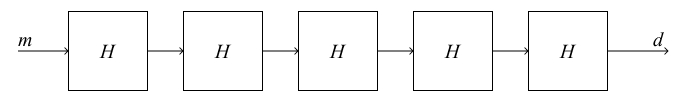
\includegraphics[width=1\textwidth]{Figures/background/hashchain_1.jpg}
  \caption[Hash chain]{}
  \label{fig:hash-chain-1}
\end{figure}

This concept was proposed by Lamport as a way to securely store passwords on servers~\cite{hashchain}. In his proposed protocol, the server just stores $H^n(p)$, where $p$ is the password and $n$ is relatively big number (for example, 1000). When the user wants to authenticate, she sends $H^{n-1}(p)$ and the server computes $H(H^{n-1}(p))$ and checks if it corresponds to $H^n(p)$. If this check succeeds, the user is authenticated and the server replace the stored value with $H^{n-1}(p)$. Next time she wants to authenticate again, she'll need to send $H^{n-2}(p)$ and this value will be checked against the previously sent digest $H^{n-1}(p)$. In this protocol, even if the transmission or the storage of the password is not secure, the user is safe.

Blockchain technology uses this idea to form the immutable chain of blocks: each block contains the hash of the previous one. Modifying a block would result in changing its hash, this would break the chain since all the following blocks would have to be recomputed, changing each digest. As shown in \ref{fig:hash-chain-2}, it's a slightly different concept than the plain hash chain, since on each step, the hashing is done on the previous digest linked to raw data of the current block, so $d_{n}=H(b_n~||~d_{n-1})$

\begin{figure}[H]
  \centering
  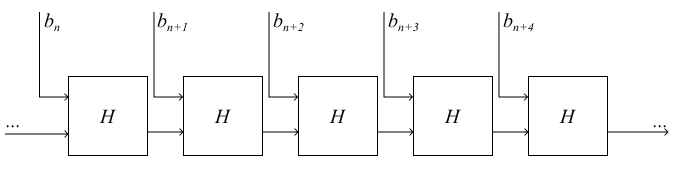
\includegraphics[width=1\textwidth]{Figures/background/hashchain_2.jpg}
  \caption[Hash chain in blockchain]{}
  \label{fig:hash-chain-2}
\end{figure}

\subsection{Merkle trees}

A Merkle tree is a data structure that generalizes the hash chain to efficiently prove membership of data. It's a binary tree in which each leaf node represents the hash of data, while intermediate nodes are computed as the hash of the two child nodes. Figure \ref{fig:merkle-tree} is an example of a Merkle tree with 4 leaf nodes.

\begin{figure}[H]
  \centering
  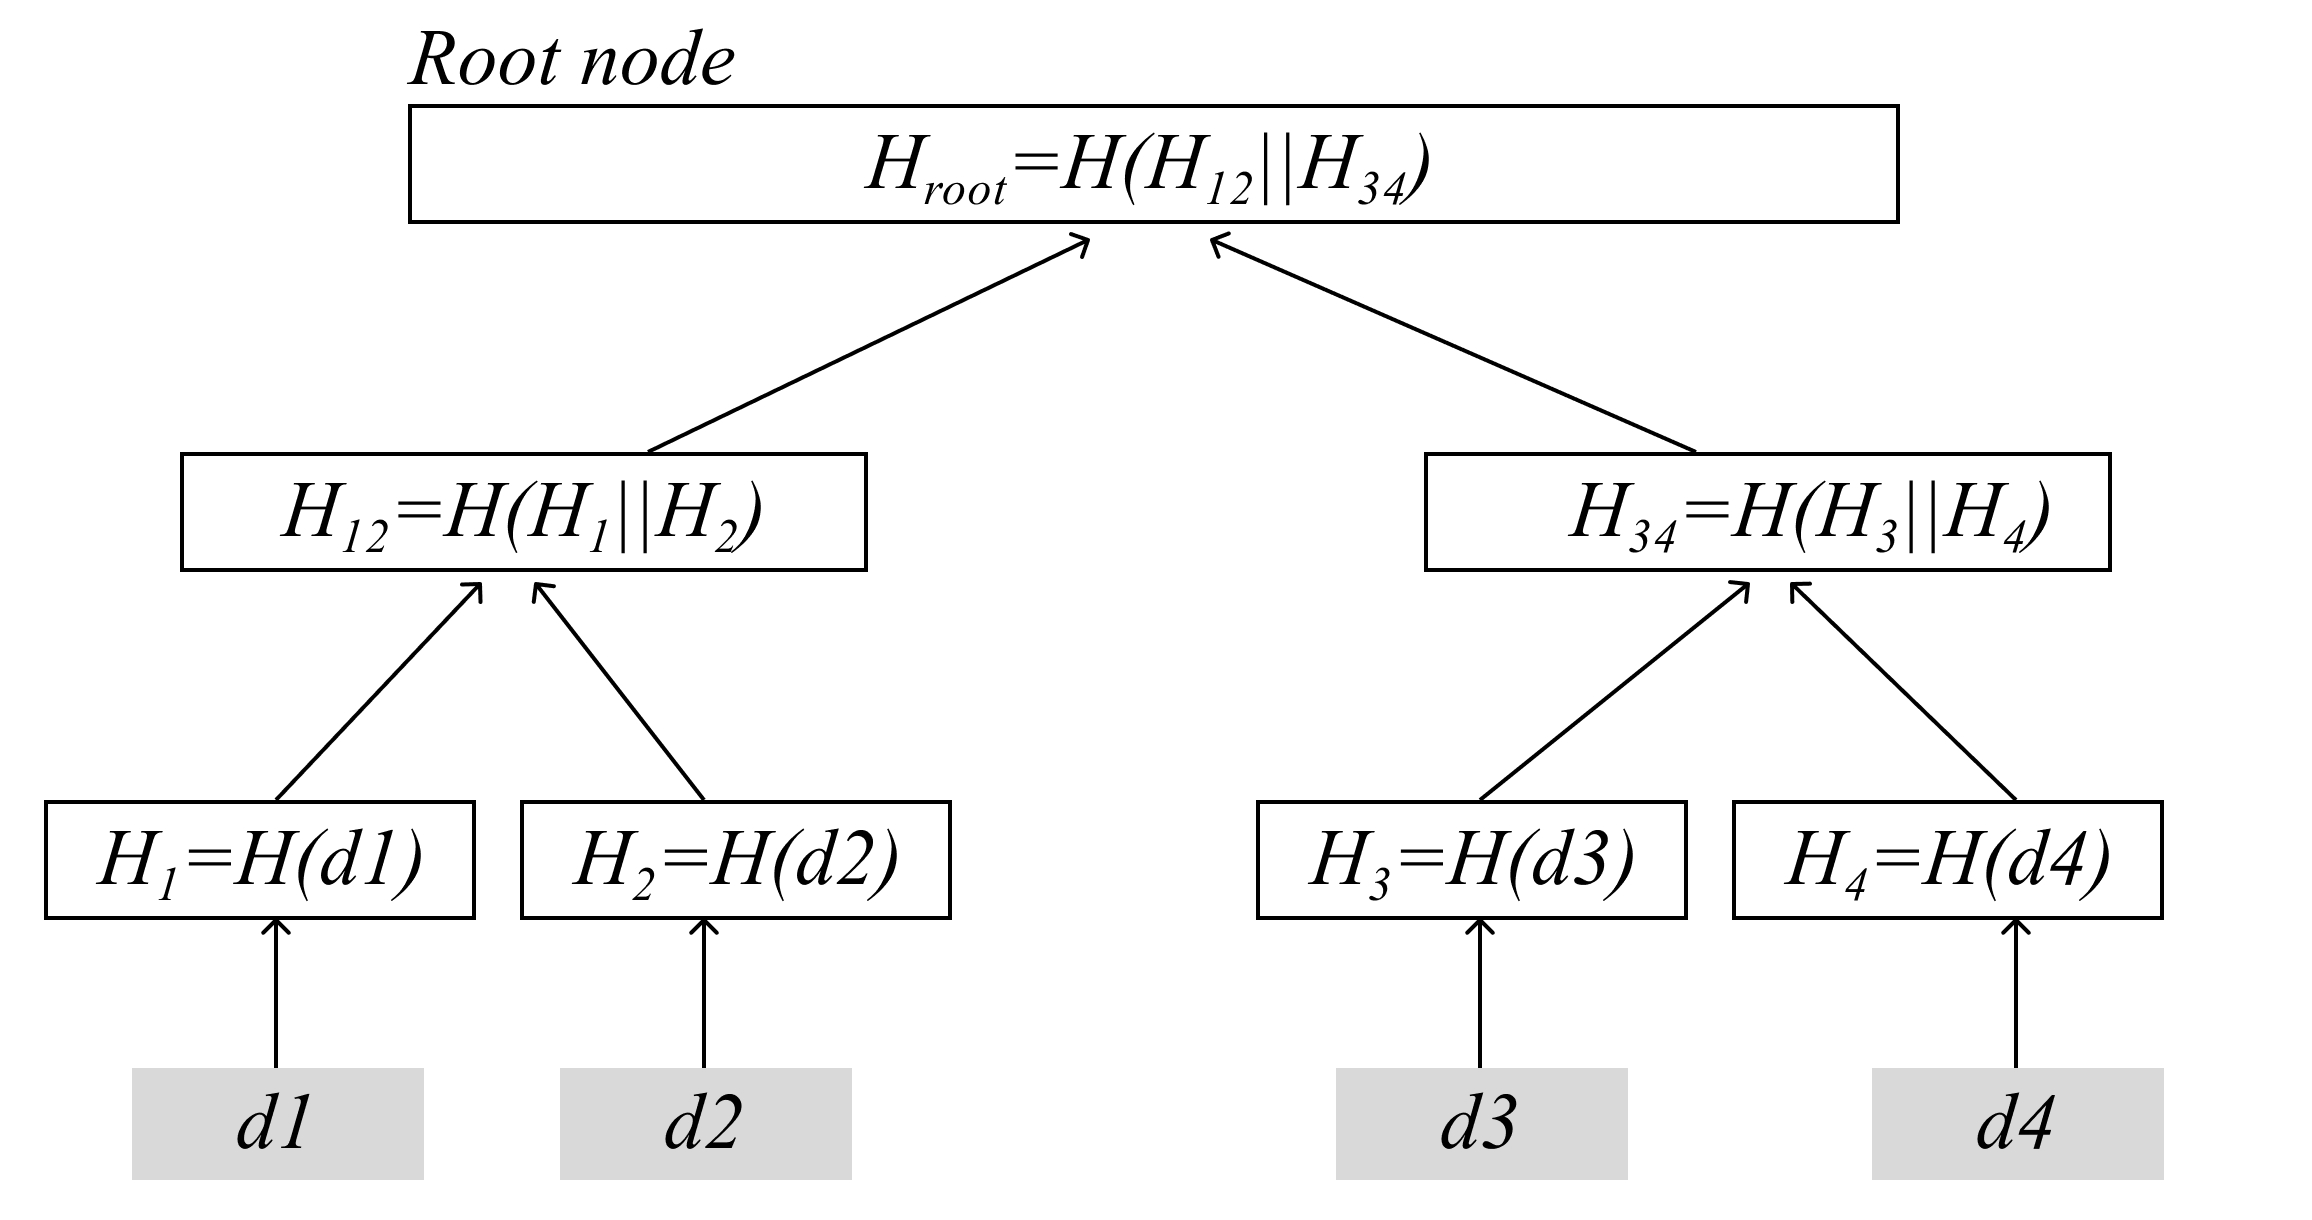
\includegraphics[width=1\textwidth]{Figures/background/merkle_tree.jpg}
  \caption[Merkle tree]{}
  \label{fig:merkle-tree}
\end{figure}

Proving membership of data to a tree with $2^n$ leaves just requires $n$ steps and $n$ intermediate nodes. The algorithm simply reconstructs the tree starting from the node that must be checked, recalculating again the root node. Data is proved to be part of the tree if the recalculated root node is equal to the given root node of the tree.

\subsection{Digital signatures}


\section{The blockchain}

What problem it's solving

\subsection{Double spending problem}

\subsection{Blockchain properties}

\subsection{Consensus layer}

\subsubsection{Proof of work}

\subsubsection{Proof of Stake}

\subsection{51\% attack}

\section{Ethereum}

\subsection{Ethereum as a state machine}

\subsection{Ethereum node}

\subsection{Smart Contracts}

\subsection{EVM}

\subsection{Solidity}

\subsection{ERC20 and ERC721}

% Eventually talk about Dgraph

% section{Graph databases}

% \subsection{Dgraph}




\cleardoublepage


\chapter{Previous work}

Data extraction and indexing from various blockchains is an essential topic for making Web3 and dApps working, there are different projects that have tried to address this problem. A lot of work has been done by companies, whose source code and methodology are not publicly available. There are also some open source or academic attempts that I will use as a comparison with my work. \\

\noindent These projects target three main categories:

\begin{itemize}
  \item Web3 and dApps developers, that need data to feed their applications.
  \item Data analysts, that need to analyse historical blockchain data. 
  \item Blockchain users, that need to see the results of transactions.
\end{itemize}

\noindent In the next sections I'll list the state of the art tools available.

\section{Etherscan}

Etherscan \footnote{https://etherscan.io/} is the reference point for accessing data about the Ethereum blockchain. It’s the most used explorer that lets people browse historical data trough a web interface. Here users can easily explore transactions, internal calls, token transfers and everything else related to the Ethereum protocol. It’s useful for inspecting singular operations, but it can’t be used for large scale analysis.

One of the most important service they offer is the verification of smart contracts, they host 461,261\footnote{This data was calculated using the CSV file exported from https://etherscan.io/chart/verified-contracts} source codes (as of 17 May 2023) that have been verified to match exactly the deployed bytecode on the  Ethereum chain. 

The process of verification consists in providing Etherscan the exact source code of a Smart Contract, the version of the compiler used, the license selected and the contract address to verify. With this information, Etherscan will try to compile the given data and check if the resulting bytecode equals the one deployed on the blockchain. There are plugins for the most used development tools like Remix or Hardhat that ease this process of verification.

This data is extremely helpful for understanding the semantic of the code deployed, since it's very hard to get useful insights by just looking at the raw bytecode. Many studies are based on these verified contracts.

Etherscan has evolved from being just an Ethereum explorer. They used the huge amount of data they have to create API endpoints and offer these data to users for a fee. These API endpoints include the standard Ethereum JSON-RPC interface and many more advanced methods, like tokens logic and specific indexes not supported by the standard RPC. 

On top of that, they also provide live and interactive charts\footnote{Available at https://etherscan.io/charts} about historical Ethereum data.

The same company that is behind the Ethereum Etherscan explorer applied the same logic and technology to other EVM compatible chains, like Polygon\footnote{https://polygonscan.com/} or BNB Smart Chain\footnote{https://bscscan.com/}.

It's important to note that, although they provide almost all the possible available Ethereum data, they haven't shared technical details about how this data is extracted or how it is indexed, users need to trust the company. Another problem is that using their data via the API for large scale analysis is unfeasible since it would be too expensive.


\section{The Graph}

The Graph~\cite{the-graph} is a decentralized indexing protocol for blockchain data. It allows users to get structured on-chain data from other users via a GraphQL\footnote{GraphQL is an open source query language created by Facebook.} interface. 

All the data is organized is so called \textbf{subgraphs} that are independent data collections that index a small subset of a blockchain network. A common pattern is that a subgraph indexes data from one or a set of few smart contracts all part of a common protocol, like Uniswap\footnote{\url{https://uniswap.org/}}. All the available subgraphs can be found on the explorer\footnote{https://thegraph.com/explorer}.

The underlying protocol is composed of multiple actors:

\begin{itemize}
  \item Developers: people with technical knowledge that develop the needed code for creating and maintaining the indexes. As of now, the most important pieces of code needed are the mappings from Ethereum events to the stored data (written in AssemblyScript\footnote{https://www.assemblyscript.org/}, a Typescript-like language that is compiled to WebAssembly) and the subgraph manifest, a structured description of all the parts needed by the subgraph in YAML format.  
  \item Indexers: they are responsible for operating a node, this implies indexing the data following a subgraph specification and serving queries.
  \item Curators: they are in charge of finding the best subgraphs to be indexed.
  \item Delegators: they secure the network by locking economical value to certain indexers they choose, giving them the possibility to serve more queries.
\end{itemize}

All these actors are economically motivated to perform well, this is achieved via a token economy where the GRT is the currency. It is implemented on the Ethereum chain with a standard ERC20 smart contract\footnote{https://etherscan.io/token/0xc944e90c64b2c07662a292be6244bdf05cda44a7}.

In order to index and serve queries, indexers have to stake at least 100,000 GRT tokens (roughly equal to 12K USD with the current change). These tokens can be slashed in case the indexer behaves maliciously. The more tokens the indexer stakes and the more queries it can serve. At the same time, indexers are rewarded with GRT tokens in two ways: query fees and annual rewards based on amount of queries served.

According to the specification of the subgraph file\footnote{https://github.com/graphprotocol/graph-node/blob/master/docs/subgraph-manifest.md\#15-data-source}, the only allowed source of data are Ethereum contracts and mappings are restricted to Events. Image \ref{fig:the-graph-data-flow} shows the flow of data in the protocol. In most cases, this is enough for dApps, since typically all the smart contracts are written in such a way that they emit events when things happen. 

On the other hand, it is not possible to index all the other kind of information for performing other analysis, such as block data, contract deployments, transactions, contracts destruction, etc. It is also not possible to extract data that was not meant to be extracted, since the emitted events are pieces of information that the developers of the smart contracts explicitly wanted to expose and index. 


\begin{figure}[H]
  \centering
  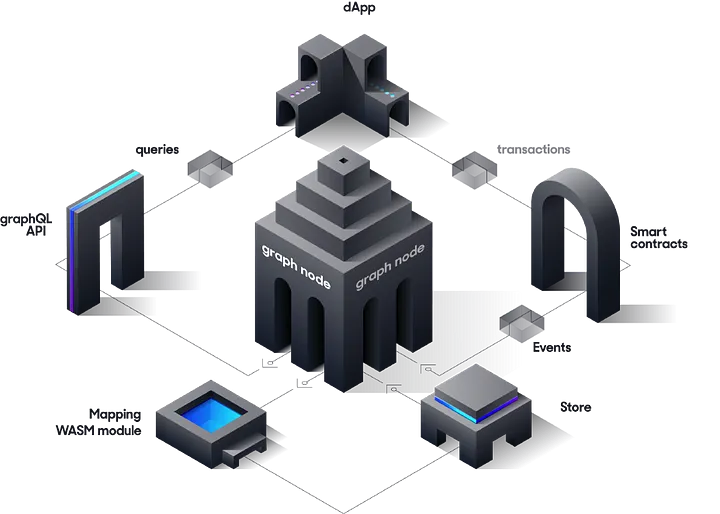
\includegraphics[width=1\textwidth]{Figures/graph-dataflow.png}
  \caption[The Graph data flow]{Data flow of The Graph indexing protocol\protect\footnotemark.}
  \label{fig:the-graph-data-flow}
\end{figure}

\footnotetext{Source: https://thegraph.com/docs/en/about/}


As of today, the protocol still relies on a central hosted service that uses the subgraphs logic and code to index data, but queries are served from this centralized server for free. This should change in 2023, the network should slowly migrate from this centralized service to the decentralized protocol once the quality of the service will be comparable \footnote{https://thegraph.academy/developers/sunsetting-the-hosted-service/}.

The Graph is the first attempt to decentralize indexing of blockchain data, it's still a project with a lot of work behind the scene. It's the most promising mechanism to make Web3 and dApps not dependant from centralized data ingestion services.


\section{Ethereum-ETL}

Ethereum-ETL\footnote{https://github.com/blockchain-etl/ethereum-etl} is an open source tool for extracting data from the Ethereum blockchain following the \textbf{Extract-Transform-Load} pattern. It's written in Python and can be used trough a CLI.

\noindent Raw data can be extracted to CSV or JSON files using these commands:

\begin{itemize}
    \item \verb|export_blocks_and_transactions|: it calls \verb|eth_getBlockByNumber| RPC and maps the response to two files containing blocks and transactions.
    \item \verb|export_token_transfers|: it calls \verb|eth_getFilterlogs| applying a filter with the first topic set to \verb|0xddf252...23b3ef|, the Keccak-256 hash of the ERC20 and ERC721 Transfer event signature. Transfers are stored in a single file without distinction between ERC20 or ERC721.   
    \item \verb|export_traces|: it stores the internal transactions calling the \verb|trace_block| method.
\end{itemize}

\noindent All other kind of data can be extracted starting from the files that these previous commands store. It is possible to further extract:

\begin{itemize}
    \item Transaction receipts and logs starting from transaction hashes exported from \verb|export_blocks_and_transactions|.
    \item Contracts data, starting from the traces stored with \verb|export_traces|.
    \item Token contracts with metadata, starting from contracts (this requires two previous step of extraction). 
\end{itemize}

\subsection{Google BigQuery public dataset}

\noindent Ethereum-ETL also allows for streaming these data from an Ethereum node to the console. This functionality is used to ingest data into the popular Ethereum Google BigQuery public dataset\footnote{https://cloud.google.com/blog/products/data-analytics/ethereum-bigquery-public-dataset-smart-contract-analytics}. This dataset is organized in six tables that I'll report here since it's a good representation of the raw data that can be extracted from an Ethereum node.

\begin{table}[H]
\centering
    \begin{tabular}  { m{6cm} m{3cm} m{3cm} } 
    \toprule
    \textbf{Attribute} & \textbf{Type} & \textbf{Required} \\
    \midrule
    timestamp & Timestamp & Yes\\ %& The timestamp for when the block was collated	\\
    number & Integer & Yes\\ %& & The block number \\
    hash & String & Yes\\ %& & Hash of the block \\
    parent\_hash & String & No\\ %& & Hash of the parent block\\
    nonce & String & Yes\\ %& Hash of the generated proof-of-work \\
    sha3\_uncles & String & No\\ %& & SHA3 of the uncles data in the block \\
    logs\_bloom & String & No\\ %& & The bloom filter for the logs of the block \\
    transaction\_root & String & No\\ %& & The root of the transaction trie of the block \\
    state\_root& String & No\\ %& & The root of the final state trie of the block \\
    receipt\_root & String & No\\ %& & The root of the receipts trie of the block \\
    miner & String & No\\ %& & The address of the beneficiary to whom the mining rewards were given \\
    difficulty & Numeric & No\\ %& & Integer of the difficulty for this block\\
    total\_difficulty & Numeric & No\\ %& & Integer of the total difficulty of the chain until this block\\
    size & Integer & No\\ %& & The size of this block in bytes\\
    extra\_data & String & No\\ %& & The extra data field of this block\\
    gas\_limit & Integer & No\\ %& & The maximum gas allowed in this block\\
    gas\_used & Integer & No\\ %& & The total used gas by all transactions in this block \\
    transaction\_count & Integer & No\\ %& & The number of transactions in the block \\
    base\_fee\_per\_gas & Integer & No\\ %& & Protocol base fee per gas, which can move up or down \\
    withdrawals\_root & String & No\\ %& & The root of the withdrawal trie of the block\\
    withdrawals & Record & Repeated\\ %& & Validator withdrawals \\
    \quad- index & \quad- Integer & \quad- No\\ %& &  \\
    \quad- validator\_index & \quad- Integer & \quad- No\\ %& & \\
    \quad- address & \quad- Integer & \quad- No\\ %& & \\
    \quad- amount & \quad- Integer & \quad- No\\ %& & \\
    \bottomrule
\end{tabular}
\caption[Google BigQuery \texttt{Blocks} table]{Description of table Blocks on the Google BigQuery public dataset, from the official docs.}
\label{table:bigquery-blocks}
\end{table}

\begin{table}[H]
\centering
    \begin{tabular}  { m{6cm} m{3cm} m{3cm} } 
    \toprule
    \textbf{Attribute} & \textbf{Type} & \textbf{Required} \\
    \midrule
    log\_index & Integer	& Yes \\
    transaction\_hash & String & Yes \\
    transaction\_index & Integer & Yes	\\		
    address & String & No \\
    data & String & No \\
    topics & String & Repeated \\
    block\_timestamp & Timestamp & Yes \\ 
    block\_number & Integer & Yes \\
    block\_hash & String & Yes \\
    \bottomrule
\end{tabular}
\caption[Google BigQuery \texttt{Logs} table]{Description of table Logs on the Google BigQuery public dataset, from the official docs.}
\label{table:bigquery-logs}
\end{table}

\begin{table}[H]
\centering
    \begin{tabular}  { m{6cm} m{3cm} m{3cm} } 
    \toprule
    \textbf{Attribute} & \textbf{Type} & \textbf{Required} \\
    \midrule
    address & String & Yes \\
    bytecode & String & No \\
    function\_signature & String & repeated \\
    is\_erc20 & Boolean & No \\
    is\_erc721 & Boolean & No \\
    block\_timestamp & Timestamp & Yes \\
    block\_number & Integer & Yes \\
    block\_hash & String & Yes \\
    \bottomrule
\end{tabular}
\caption[Google BigQuery \texttt{Contracts} table]{Description of table Contracts on the Google BigQuery public dataset, from the official docs.}
\label{table:bigquery-contracts}
\end{table}

\begin{table}[H]
\centering
    \begin{tabular}  { m{6cm} m{3cm} m{3cm} } 
    \toprule
    \textbf{Attribute} & \textbf{Type} & \textbf{Required} \\
    \midrule
    transaction\_hash & String &	No	\\			
    transaction\_index & Integer	& No	\\			
    from\_address & String &	No \\	
    to\_address & String & No \\				
    value & Numeric &	No		\\		
    input & String &	No		\\		
    output & String	& No		\\		
    trace\_type & String &	Yes		\\		
    call\_type & String	& No	\\
    reward\_type & String	& No\\
    gas & Integer	& No\\
    gas\_used & Integer	& No\\
    subtraces & Integer	& No\\
    trace\_address & String	& No		\\
    error & String	& No		\\
    status & Integer	& No	\\		
    block\_timestamp & Timestamp	& Yes		\\		
    block\_number & Integer	& Yes			\\	
    block\_hash & String	& Yes	\\			
    trace\_id & String	& No \\
    \bottomrule
\end{tabular}
\caption[Google BigQuery \texttt{Traces} table]{Description of table Traces on the Google BigQuery public dataset, from the official docs.}
\label{table:bigquery-traces}
\end{table}

\begin{table}[H]
\centering
    \begin{tabular}  { m{6cm} m{3cm} m{3cm} } 
    \toprule
    \textbf{Attribute} & \textbf{Type} & \textbf{Required} \\
    \midrule
    token\_address & String & Yes	 \\			
    from\_address & String & No \\
    to\_address & String	& No	\\			
    value & String	& No	\\
    \bottomrule
\end{tabular}
\caption[Google BigQuery \texttt{Token\_transfers} table]{Description of table Token\_transfers on the Google BigQuery public dataset, from the official docs.}
\label{table:bigquery-transfers}
\end{table}

\begin{table}[H]
\centering
    \begin{tabular}  { m{6cm} m{3cm} m{3cm} } 
    \toprule
    \textbf{Attribute} & \textbf{Type} & \textbf{Required} \\
    \midrule
    hash & String	& Yes		\\		
    nonce & Integer	& Yes \\				
    transaction\_index & Integer	& Yes		\\		
    from\_address & String	& Yes			\\	
    to\_address & String	& No		\\		
    value & Numeric	& No \\				
    gas &  Integer	& No \\				 
    gas\_price &  Integer &	No \\				
    input &  String	& No \\				
    receipt\_cumulative\_gas\_used & Integer & 	No \\				
    receipt\_gas\_used  & Integer	& No \\				
    receipt\_contract\_address & String	& No \\				
    receipt\_root &  String & 	No \\				
    receipt\_status  & Integer & 	No \\				
    block\_timestamp  & Timestamp	 & Yes \\				
    block\_number  & Integer & 	Yes \\				
    block\_hash & String &	Yes \\				
    max\_fee\_per\_gas & Integer	& No \\	
    max\_priority\_fee\_per\_gas & Integer	& No \\		
    transaction\_type & Integer	& No				\\
    receipt\_effective\_gas\_price & Integer	& No	\\
    \bottomrule
\end{tabular}
\caption[Google BigQuery \texttt{Transactions} table]{Description of table Transactions on the Google BigQuery public dataset, from the official docs.}
\label{table:bigquery-transactions}
\end{table}

It is possible to query these tables using SQL syntax, they can be joined on equal fields. There is the possibility to query this database for free up to a certain monthly limit of processing storage and amount of data extracted. 

I'll compare Ethereum-ETL with my work in the next chapters.

\section{Dune analytics}

Dune Analytics\footnote{https://dune.com/home} is a company that provides tools to query and visualize data from multiple blockchains. They support Bitcoin, Solana, Ethereum and other 8 EVM chains.\\

Their application is web-based, from there it is possible to create queries using SQL syntax and visualize results in interactive charts. Multiple queries can be collected together to create dashboards\footnote{Example of a dashboard about history of Ethereum: https://dune.com/hildobby/ethereum}.  

\subsection{Data architecture}

Blockchain data was initially managed using PostgreSQL and SparkSQL until 2022, year in which they released their own engine called DuneSQL \footnote{https://dune.com/blog/dune-engine-v2}, migration to this technology is currently ongoing. \\

They started storing and indexing data with PostgreSQL.
In this DBMS entries are stored in pages following a row-oriented strategy, which means that all the attributes of a row are stored adjacently. This is beneficial when it's necessary to retrieve all the attributes of a row while querying. However, it leads to poor performance when filtering for specific attributes, since the database has to load many bytes containing irrelevant data (i.e., all the other attributes of the row that are not used). To optimize this, it is possible to create indexes on columns. These indexes will provide very good performance, but can be hard and slow to maintain, specially with huge amount of data. At Dune Analytics they tried this approach with traditional relational database combined with indexes, but they had to drop it stating that "the size of the datasets were so huge that the database was struggling to fully support them"\footnote{Source: https://dune.com/blog/introducing-dune-sql}. \\

So they came up with DuneSQL, a query engine built specifically for managing blockchain data. It's a fork of Trino, an open source distributed SQL query engine designed to query data from heterogeneous sources. The DuneSQL fork is not open source, so technical information can only be deducted from their blog articles or statements on the support community. The main features they added are \textit{varbinary} data type for storing addresses and hashes, as well as \textit{uint256} support for EVM data. \\

Data is physically stored on AWS S3 buckets using the Apache Parquet storage format\footnote{https://github.com/apache/parquet-format}. This storage system is a mix between column and row oriented. Data is split in files based on rows, inside these files, there are further row groups and inside these groups data is divided by columns. Image \ref{fig:parquet-structure} visualize this concept. \\

\begin{figure}[H]
  \centering
  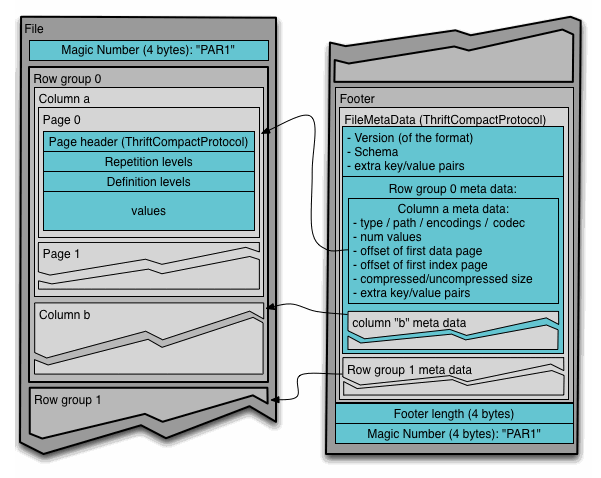
\includegraphics[width=1\textwidth]{Figures/parquet-structure.png}
  \caption[Parquet storage format structure]{File structure in the Parquet storage format\protect\footnotemark.}
  \label{fig:parquet-structure}
\end{figure}

\footnotetext{Source: https://github.com/apache/parquet-format}

Indexing is done using the Parquet file's metadata. At the end of each file there's a part in which are stored min/max values of all the column values inside a page, as shown in image \ref{fig:parquet-index}. This information allows the database to skip reading the whole chunk if values are not in the desired range. While working great for certain types of data, it isn't very useful with strings, especially if they are not sorted. That's the reason why even a simple query like \ref{lst:dune-query} can take several minutes to run. \\

\begin{figure}[H]
  \centering
  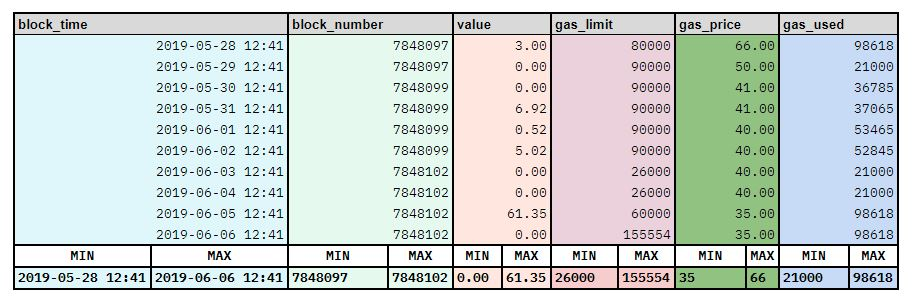
\includegraphics[width=1\textwidth]{Figures/parquet-index.jpg}
  \caption[Parquet ColumnIndex on Dune Analytics]{Parquet min/max column index structure \protect\footnotemark. }
  \label{fig:parquet-index}
\end{figure}

\footnotetext{Source: https://dune.com/docs/query/storage/}

\begin{lstlisting}[language=SQL,caption={Shortened simple query on DuneSQL that took 3 minutes to run},label={lst:dune-query},captionpos=b]
Select * from ethereum.transactions
where hash = 0x9ef65fe51...ff74219e
\end{lstlisting}

\subsection{Available data}

On Dune Analytics, blockchain data is available in multiple layers:

\begin{itemize}
    \item \textit{Raw tables}: these tables contain raw data as it is stored on the various blockchains, without modifications. For EVM chains this means Blocks, Logs, Traces and Transactions.
    \item \textit{Decoded tables}: verified contracts receive their own tables on which data is stored in a more readable way. Each event and function that is present in the contract's ABI corresponds to a table on Dune with the following name pattern: \texttt{project\_chain.contract\_[evt/call]\_evtOrCallName}. Inside this table there will be columns for each of the event or function attributes, with the relative names. For example, all the \textit{cryptokitties} \texttt{Transfer} events are stored in a table called \texttt{cryptokitties\_ethereum.KittyCore\_evt\_Transfer} that will have, among other contextual information, three columns: \textit{from}/\textit{to} addresses and \textit{tokenId}.
    \item \textit{Spellbooks}: these tables are abstractions over raw and decoded data that give users an easy way to retrieve information without diving into the technicalities of complex decentralized protocols. They're open source and the community can contribute creating new spellbooks on the Github Repository\footnote{https://github.com/duneanalytics/spellbook}. The main power of spellbooks is to put together data from heterogeneous sources to gather useful insights. The most clear example is the \texttt{dex.trades}\footnote{https://github.com/duneanalytics/spellbook/blob/main/models/dex/dex\_trades.sql} spellbook, that puts together all the trades made on all decentralized exchanges of all the blockchains present on Dune Analytics.
\end{itemize}

\section{XBlock-ETH}

Zheng et al.~\cite{xblock-eth} released a dataset containing raw Ethereum data and described the framework used for getting it, called XBlock-ETH. It was released in 2019 and data is periodically updated in chunks of 500,000 blocks, currently it covers blocks from 0 to 16,499,999. It is divided in different smaller datasets: \textit{Block}, \textit{Block Transaction}, \textit{Internal Transaction}, \textit{Contract Info}, \textit{ERC20 Transaction}, \textit{ERC721 Transaction}, \textit{Token Info}. Data can be downloaded from their website\footnote{https://xblock.pro/xblock-eth.html} in CSV format.

This is a useful resource for getting Ethereum data without having the possibility to run a node; however it lacks important information such as logs and receipts. 

It's not easy to use, since the massive amount of data in the CSV files must be parsed and cannot be easily queried or indexed, further transformation steps are needed. There are some Python scripts available on Github\footnote{https://github.com/tczpl/XBlock-ETH} for downloading and analysing the data, but the code used for the extraction is not open source, so it's not possible to know exactly how information was retrieved.

\section{Data-ether}

DateEther \cite{dataether} is a framework presented by Chen et al. for extracting and indexing Ethereum data. They tried a different approach for executing this task: they modified a Geth\footnote{https://geth.ethereum.org/} node to record and store data during the initial synchronization phase. They used ElasticSearch\footnote{https://www.elastic.co/} for indexing and exploring data, but by the time of their research the size of data was relatively small compared to now.

While extracting data by modifying a node source code was efficient back in 2019, now Ethereum nodes have evolved and there are different and faster RPCs for getting internal transactions. Their way of extracting data was compared against \texttt{debug\_traceTransaction} RPC of Geth, claiming to be 18.6x faster, but it wasn't compare against \texttt{debug\_traceBlock} or \texttt{trace\_block} of Erigon\footnote{https://github.com/ledgerwatch/erigon}. From my work, using Erigon's \texttt{trace\_block} RPC, I managed to get and loop trough all the internal transactions in around 9 hours (40 including transactions and logs). Doing that while synchronizing a node would have required at least 3-4 days. 

Extracting data by modifying source code has another drawback: maintainability. Just Geth itself received 173 releases\footnote{https://github.com/ethereum/go-ethereum/releases}, modifying its source code would mean having to merge the code and resolving eventual conflicts every time a new release is published. This is not a problem using Ethereum RPC APIs since they don't change after upgrades of the nodes.

\section{Web3 providers}

The term "Web3 provider" is commonly used to refer to companies that offer access to Ethereum RPC API, avoiding developers of Web3 dApps the costs of running a node. They're included in this chapter since the majority of them also provide access to indexed and interpreted data. Some popular web3 providers include Alchemy\footnote{https://www.alchemy.com/}, Infura\footnote{https://www.infura.io/}, Quicknode\footnote{https://www.quicknode.com/} and Chainstack\footnote{https://chainstack.com/}.

All of them have endpoints for getting NFTs data, it's possible to get all NFTs owned by an address by just calling an API instead of having to analyze all the chain. Chainstack also hosts on their servers all the supgraphs of "The Graph" protocol, offering users the possibility to use a more stable service instead of the decentralized alterntive.

It is important to note that the web3 providers are profit-oriented companies. While they provide an important service in the world of dApps, it's essential to consider their cost implications. Using their services for analyzing historical data can be very expensive, since billing is done based on number of API requests to their server.

Another important aspect to consider is the transparency of these services. As profit-oriented entities, these web3 providers do not necessarily make their source code and methodology open source. This means that developers relying on their services need to trust the data they receive. 

Depending on centralized companies poses also a risk to the actual decentralization of the web3. Access to the blockchain infrastructure is concentrated on a few companies, as noted by Wang et al.~\cite{wang2022exploring}.

\section{Comparison}

I summarized in table \ref{table:tools-comparison} the main differences between the tools in terms of \textit{primary target}, \textit{transparency} and \textit{price}.

\begin{table}[ht!]
\centering
    \begin{threeparttable}
    \begin{tabular}  { m{3cm} m{3cm} m{1.5cm} m{5cm} } 
    \toprule
    \textbf{Tool} & \textbf{Target} & \textbf{Open source} & \textbf{Price}  \\
    \midrule
    Etherscan    & Blockchain users  & No & Free explorer, paid apis  \\[2.3ex]
    The Graph     & Web3 developers & Yes & Billing based on usage  \\[1.3ex]
    Ethereum-ETL     & Data analysts & Yes & Free  \\[1.3ex]
    Dune Analytics      & Data analysts & No & Based on query credits, it has free plan \\[2.6ex]
    XBlock-ETH  & Data analysts & No\tnote{*} & Free   \\[1.3ex]
    DataEther  & Data analysts & No\tnote{*} & Free   \\[1.3ex]
    Web3 providers      & Web3 developers & No & Billing on usage, they have free plans   \\[1.6ex]
    \bottomrule
    \end{tabular}
    \begin{tablenotes}
      \item[*] Source code not available, but they released technical papers describing the software.
      \end{tablenotes}
    \end{threeparttable}
\caption[State of the art tools comparison]{Comparison of state-of-the art tools for management of blockchain data.}
\label{table:tools-comparison}
\end{table}

\cleardoublepage


\chapter{Methods}

\noindent In this chapter, I introduce {\tt eth2dgraph}, the new open-source software designed to facilitate the extraction and indexing of Ethereum data in Dgraph.

Eth2dgraph is developed using Rust, a system programming language that prioritizes both speed and safety. Rust was chosen mainly for two reasons. Firstly, for its emphasis on performance and parallelism, crucial for scaling the data extraction process and achieving good performance. Secondly, Rust benefits from a rich ecosystem of libraries specifically designed for handling Ethereum data, easing the process of development.

One of the key features of eth2dgraph is its integration with a decompiler, enabling the extraction at scale of the Application Binary Interface (ABI) from the bytecode stored on the Ethereum blockchain. 

The following sections provide details about the architecture of eth2dgraph, give a comprehensive overview of how the software operates, and how it has been constructed.

\section{Data flow}

Extracting and indexing Ethereum Smart Contract data is a process of moving and transforming bytes. Raw data stored in the Ethereum node must be taken, transformed and ingested into a database, Dgraph in this case, in order to be indexed. 

The first attempt was to do this step through transactions. I ran a Dgraph cluster and instructed eth2dgraph to add data via DQL mutations. DQL stands for \textbf{Dgraph Query Language} and it is the language used to write Dgraph queries. This data flow was working but it was too slow for thinking about applying it to all the history of the Ethereum chain. I also had problems to parallelize data insertion, too many concurrent transactions were failing due to read-write conflicts. \cref{fig:data-flow-1} visualizes this data flow.

\begin{figure}[H]
\centering
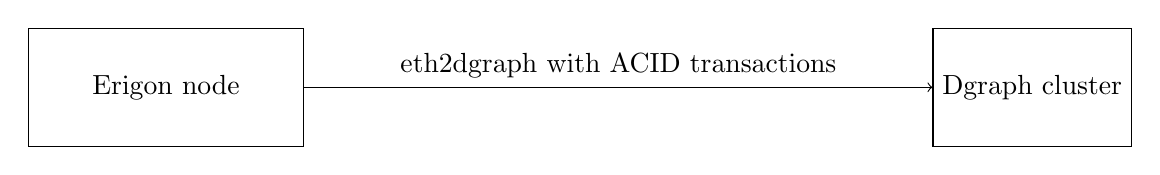
\begin{tikzpicture}
    \node[draw,minimum width=35mm,minimum height=15mm] (erigon) at (0,0) {Erigon node};
    \node[draw, minimum width=25mm,minimum height=15mm] (dgraph) at (11,0) {Dgraph cluster};
    \draw[->] (erigon) edge node[sloped, above] {eth2dgraph with ACID transactions} (dgraph);
\end{tikzpicture}
\caption[First attempt of data ingestion into Dgraph]{First attempt of data ingestion into Dgraph}
\label{fig:data-flow-1}
\end{figure}

To solve these problems, I changed the approach and followed an ETL (Extract, Transform, Load) process. Extraction and transformation are done in the same step by eth2dgraph. The output is stored in JSON files that can be later loaded into Dgraph using the Bulk Loader.

The Bulk Loader\footnote{Detailed description of the Bulk Loader: \url{https://dgraph.io/blog/post/bulkloader/}} is a tool provided by Dgraph. It is designed for performing the initial load of data into the database. It takes JSON or RDF N-Quads\footnote{N-Quads is a serialization format for RDF graphs data \url{https://www.w3.org/TR/n-quads/}.} data and stores it directly in Badger, the underlying key-value database used by Dgraph. This is the fastest way to ingest data into Dgraph. It maximizes concurrency and avoid problems related to ACID constraints since it is not operating on a live database. \cref{fig:data-flow-2} visualizes the final data flow chosen for eth2dgraph.

\begin{figure}[H]
\centering
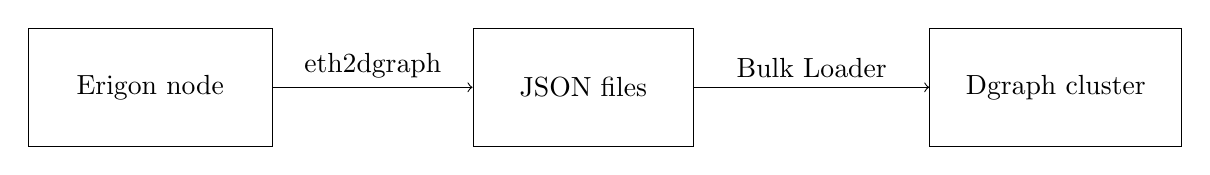
\begin{tikzpicture}
    \node[draw,minimum width=31mm,minimum height=15mm] (erigon) at (0,0) {Erigon node};
    \node[draw, minimum width=28mm,minimum height=15mm] (json) at (5.5,0) {JSON files};
    \node[draw, minimum width=32mm,minimum height=15mm] (dgraph) at (11.5,0) {Dgraph cluster};
    \draw[->] (erigon) edge node[sloped, above] {eth2dgraph} (json);
    \draw[->] (json) edge node[sloped, above] {Bulk Loader} (dgraph);
\end{tikzpicture}
\caption[Second and final data flow]{Second and final data flow}
  \label{fig:data-flow-2}
\end{figure}

\section{Data model}

After seeing how data is indexed in other works, I decided to design the schema in a slightly different way. In eth2dgraph, raw data is interpreted to create a schema around the semantics that can be extracted from the blockchain. This semantics is indexed alongside the raw Ethereum data. \cref{fig:schema} shows the whole schema that was created. All the edges have the {\tt @reverse} index, that means they can be traversed in both directions. Some of the attributes are indexed at load time, but it is easy to add indexes once the database is running. The complete description of both DQL and GraphQL schemas are described in~\cref{app-b}.

% TODO: update schema with final version

\begin{figure}[H]
  \centering
  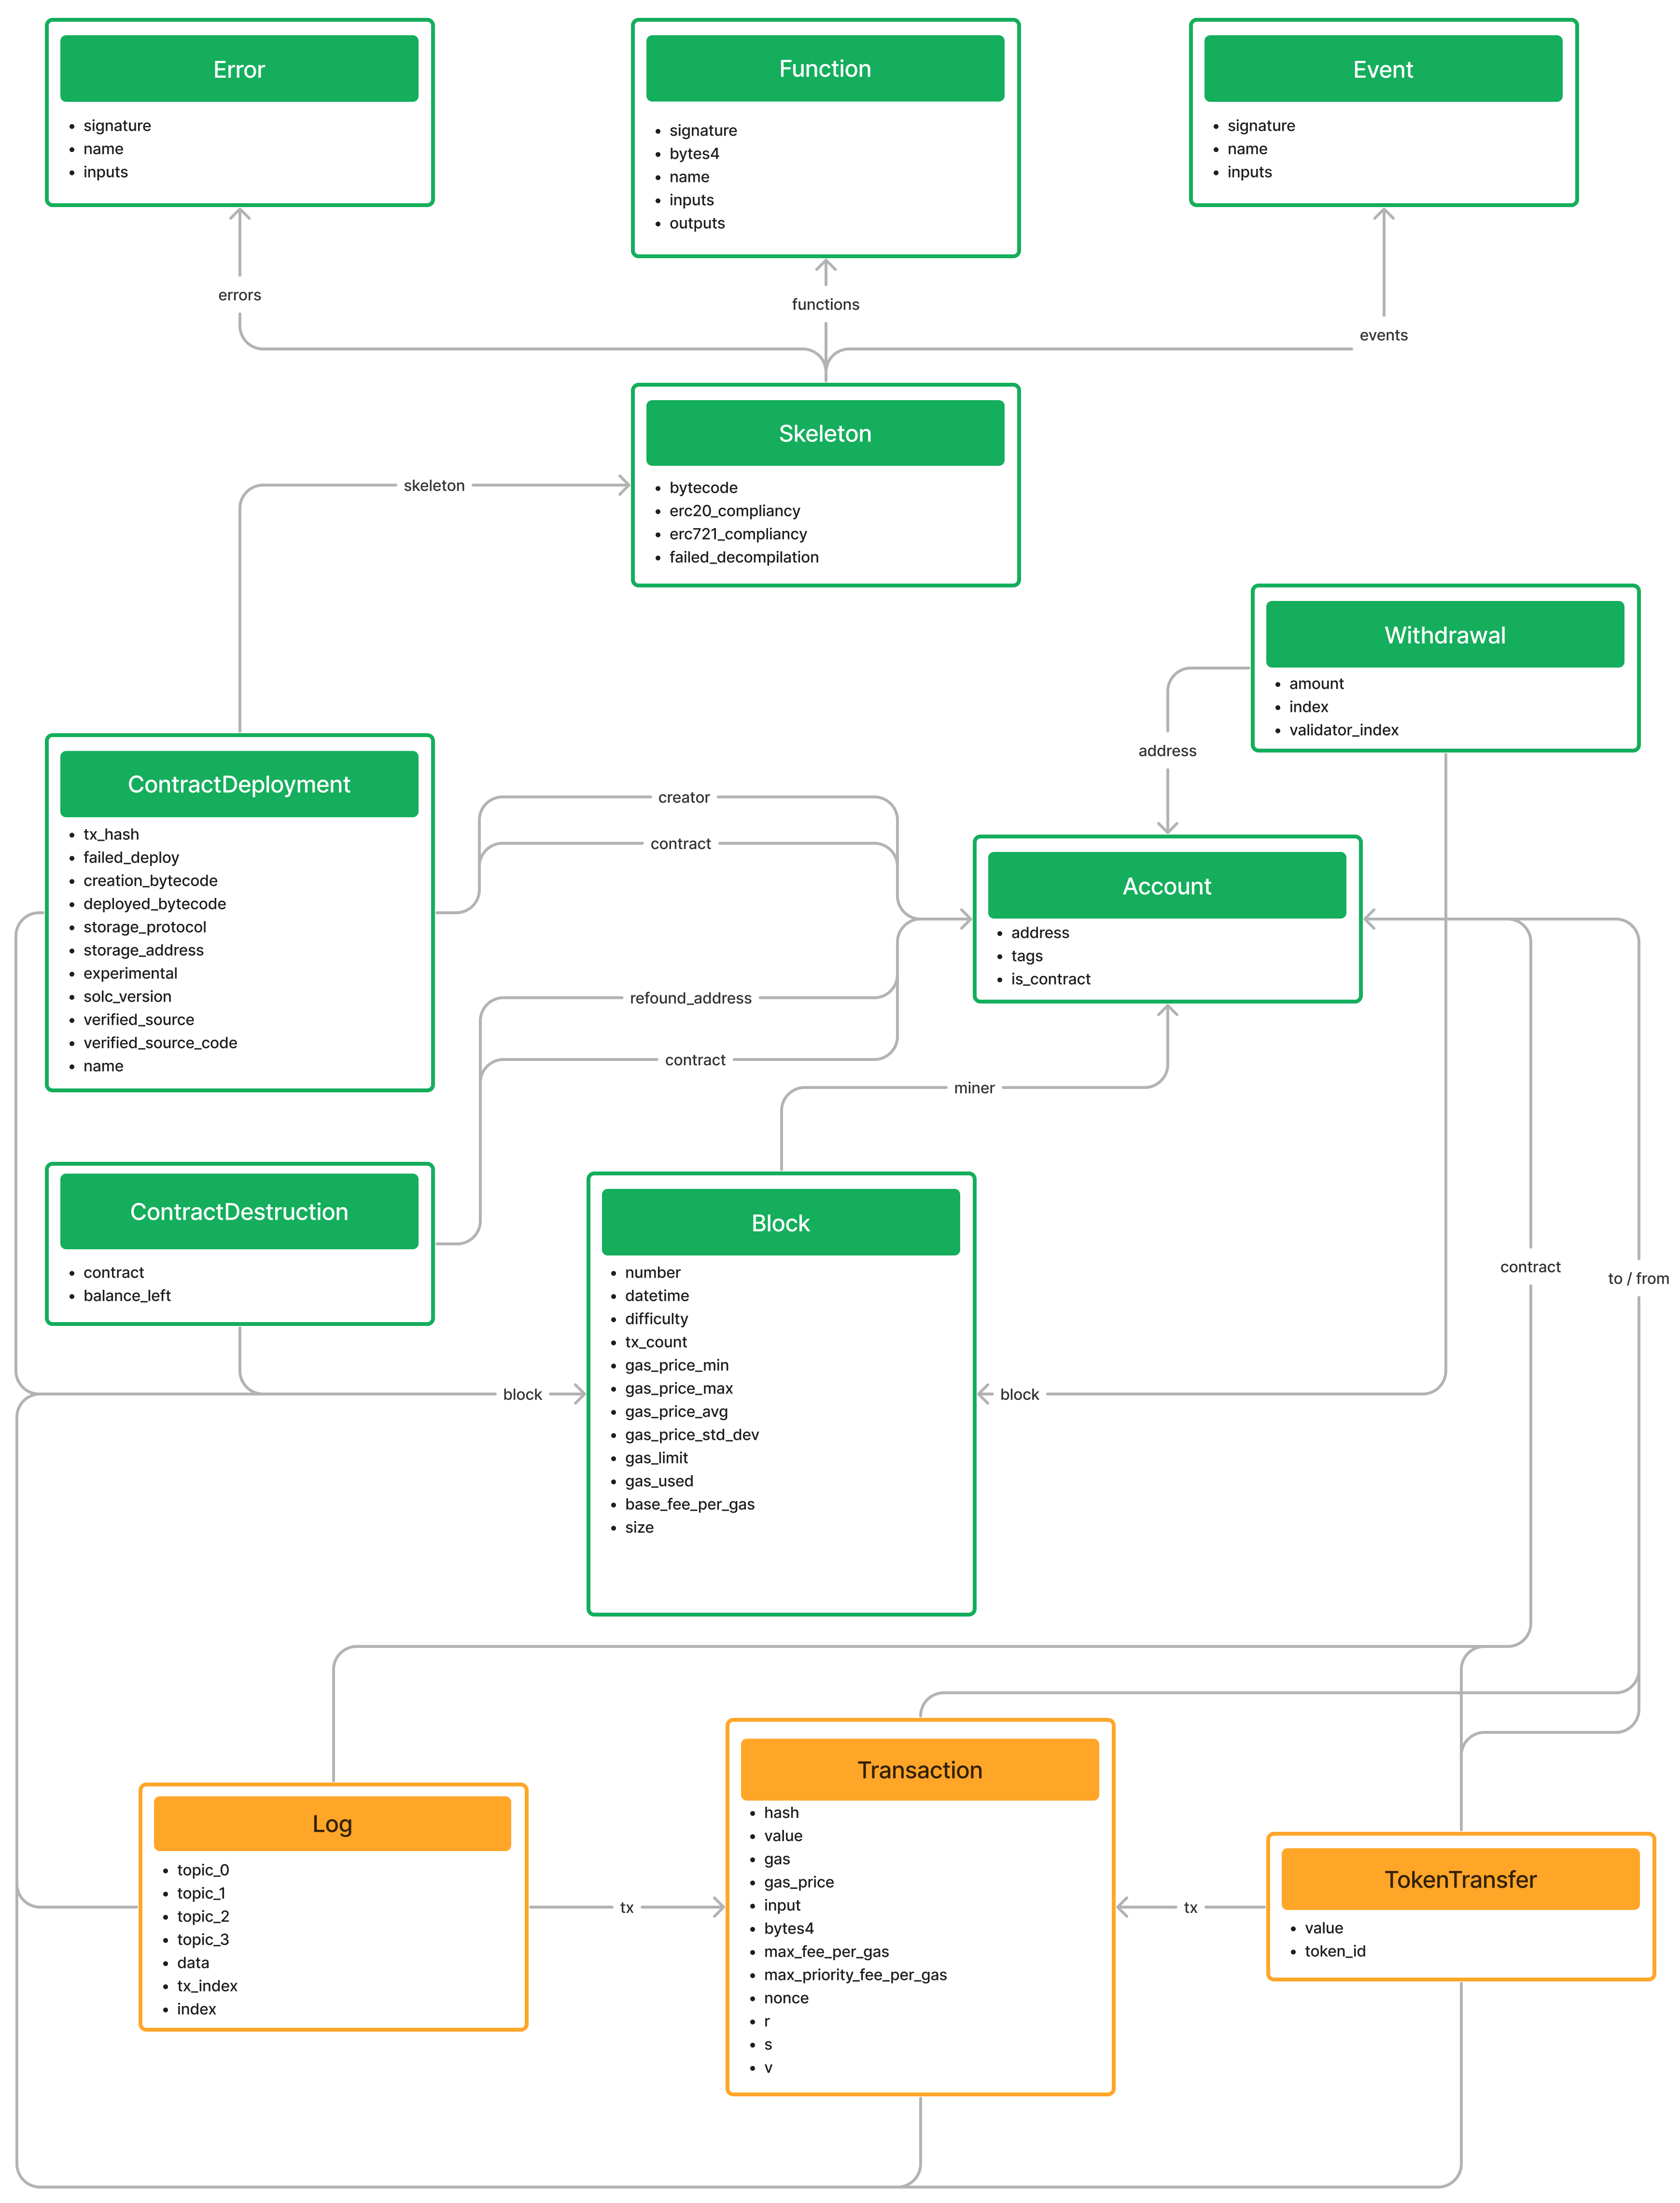
\includegraphics[width=1\textwidth]{Figures/methods/schema.png}
  \caption[Schema of Ethereum indexed data in Dgraph]{Schema of Ethereum indexed data in Dgraph}
  \label{fig:schema}
\end{figure}

Data is modeled as a graph with many edges. This was done since Dgraph is designed and optimized to perform joins and traversals.

Entities in yellow (\textit{Transaction}, \textit{TokenTransfer} and \textit{Log}), also called \textit{dynamic}, are optional and can be skipped during data extraction. Excluding data about smart contracts usage allows the creation of a much smaller dataset that provides a static description of these contracts. The reason of this choice is that the volume of dynamic data is around 30-40x bigger than static data. Having the option to extract a smaller dataset enables analysis on less powerful computers, improving the accessibility of the research. \\

\noindent Here is a brief description of the schema:

\begin{itemize}

    \item \textit{Transaction} and \textit{Log} are stored as they are retrieved from the Ethereum node. References to other entities are stored as edges for allowing graph traversal in queries. A \textit{Transaction} represents a transfer of value between two EOAs or an invocation of a Smart Contract from an EOA. A \textit{Log} is the result of an invocation of an Event in the code of a Smart Contract.

    \item \textit{TokenTransfer} represents both an ERC20 or an ERC721 token transfer between two accounts. Value is stored as a string since Dgraph does not handle 256 bit integers.
    
    \item \textit{Block} contains all the information related to a single Ethereum block. It includes data related to the withdrawals of validators. This entity is connected to many others: \textit{ContractDeployment}, \textit{ContractDestruction}, \textit{Transaction}, \textit{TokenTransfer} and \textit{Log}. 
    
    The indexed attribute \textit{datetime} is the only reference to time in the database, so it is possible to query it for specific dates and times and then get all the connected data from there. 

    \item \textit{Account} represents an Externally Owned Account or a Contract Account. Its fundamental attribute is the \textit{Address} of the account. There is also a boolean field \textit{is\_contract} indicating whether the account is a contract or not. This entity is extremely useful for querying data, since with the standard Ethereum RPC interface it is not possible to query data based on account addresses. So, for example, it is impossible to get all the transactions from/to an address without having to download and filter all the transactions in the history of Ethereum.

    \item \textit{ContractDeployment} and \textit{ContractDestruction} represent respectively the birth and the death of the code of a Smart Contract. I decided to store them in this way since I found, analyzing the data, that a single Ethereum Address can receive more than one code deployment, contrary to what it may appear because of the theoretical immutability of Smart Contracts. An address can receive both a deployment with the same old code or with new different code, in which case it is called \textit{morphic} or \textit{metamorphic}~\cite{create2-metamorphic}.

    \item I introduced the concept of \textit{Skeleton} directly in the schema since it is a useful way of aggregating similar contracts together. A \textit{Skeleton} is the bytecode of a contract without all the arguments of the PUSH opcodes. Having it directly in the schema allows to easily find contracts sharing the same skeleton.

    \item \textit{Event}, \textit{Function} and \textit{Error} are the parts that, together, form the ABI of the contracts. There is just one entity for each signature, so all the contracts implementing the same function/event/error point to the same entity. Having them indexed in this way allows to search contracts based on the functionalities they implement.
    
\end{itemize}

\section{Data extraction}

Data is extracted using the Ethereum \textit{Remote Procedure Call} (RPC) interface\footnote{Official specification of the Ethereum RPC interface: \url{https://ethereum.github.io/execution-apis/api-documentation/}}. Eth2dgraph extracts data block by block. It needs three API calls per block to get all the data: \texttt{eth\_getBlockByNumber}, \texttt{eth\_getLogs} and \texttt{trace\_block}. 

To call these RPCs, I used the library \texttt{ethers-rs}\footnote{\url{https://docs.rs/ethers/latest/ethers/}}, which provides, among other functionalities, a full client implementation in Rust that wraps the standard Ethereun interface and provides easy methods to interact with it in an asynchronous runtime.

At high level, data returned from these RPC endpoints is parsed into Rust structs and later serialized into JSON files using the \textit{serde}\footnote{Serde is a Rust framework for easily serializing and de-serializing data structures \url{https://github.com/serde-rs/serde}} crate. To implement this, all the Rust structs that must be serialized to Dgraph format implement a trait called \textit{SerializeDgraph}. In Rust, a trait defines a collection of methods. A struct that implements a trait is guaranteed to have that methods implemented. It is a concept similar to the Interfaces in object oriented programming (OOP) languages.

The trait \textit{SerializeDgraph} requires one method to be implemented:\\ \texttt{serialize\_dgraph}. As the name suggests, it is a function that serializes a generic struct to the JSON format accepted by the Dgraph Bulk Loader.

The entities produced by eth2dgraph are linked together using the Dgraph's \textit{blank nodes}. It is a way of referencing to an entity that has yet to be created. Dgraph will resolve all the references to a blank node generating and using the same \texttt{uid}.

The next sections explain how each piece of data is extracted.

\subsection{Blocks and transactions}

Blocks and transactions are both extracted from the data returned by the RPC \texttt{eth\_getBlockByNumber}. 
This method accepts two parameters:

\begin{itemize}
    \item \textit{Block number} specifies the target block that is extracted
    \item \textit{Hydrated transactions} is a boolean indicating whether to return or not all the details of the transactions in that block.
\end{itemize}

Eth2dgraph calls this RPC sequentially for each block with \textit{Hydrated transactions} set to \texttt{true}. All raw transactions data is stored without modifications, same for the withdrawals. For the blocks I added a summary about the gas price, this is not returned by  default from the RPC. These fields have been added: 

\begin{itemize}
    \item \textit{gas\_price\_min}: the cheapest gas price of all the transactions included in the block, in Gwei.
    \item \textit{gas\_price\_max}: the maximum amount paid for gas in the transactions included in the block, in Gwei.
    \item \textit{gas\_price\_avg}: the average price of gas in Gwei of that block.
    \item \textit{gas\_price\_std\_dev}: the standard deviation of gas price in that block, in Gwei.
\end{itemize}

Gas price varies between each transaction. Sticking to the official RPC docs, it should be possible to obtain data about it just from the transaction receipts. This would imply getting more data and slowing down the process of data extraction.

Looking at the data returned from the Erigon node and analyzing its source code\footnote{\url{https://github.com/ledgerwatch/erigon/blob/35422986645832d1c9ce1107a59dbaf4e12f55dd/turbo/adapter/ethapi/api.go\#L450}}, I noticed that gas price was present even if not required by the protocol. I compared it to the data returned from the receipts and it matched, so I decided to use it and store this information in the database.

\subsection{Logs}

Logs are retrieved using the \texttt{eth\_getLogs} RPC. This remote procedure call accepts an object as parameter, it can be used as a filter to refine the call and get just the logs needed. It is possible to filter by topics, contract address and blocks range. 

All the logs are already indexed in the Ethereum nodes by the fields on which it is possible to filter. It is the standard way to extract semantics from the chain. When specifics conditions happen inside a call to a smart contract, it can emit a log with up to four indexed 256 bits words that will be stored by all the Ethereum nodes. These logs can represent any kind of information, e.g.~token transfers, and token swaps.

Eth2dgraph is getting logs downloading them block by block. The RPC \textit{eth\_getLog} is called for each block with a filter on the blocks range, with matching \textit{fromBlock} and \textit{toBlock} parameters.

\subsection{Smart contracts}

There are two ways for deploying a smart contract on the Ethereum blockchain: 

\begin{itemize}
    \item From EOAs, with a transaction to the address \texttt{0x0} containing as input data the deployment code of the smart contract.
    \item From other smart contracts, calling the EVM opcode \texttt{CREATE} or \texttt{CREATE2}, after having pushed on the stack the deployment code of the smart contract to deploy.
\end{itemize}

There is no RPC to directly get the list of contracts. Smart contracts are not indexed by the Ethereum nodes.

It is relatively easy to extract smart contracts deployed in the first way, it is enough to loop trough transactions and see the ones sent to the address \texttt{0x0}. The resulting transactions are potential contract deployments. To confirm this, it is possible to download their receipts, which contain the address of the newly created contract in case the deployment is successful. After finding the address, it is possible to get the deployed bytecode calling the RPC \texttt{eth\_getCode}, which returns the actual code stored on the blockchain.

This way of extracting contracts has two drawbacks: it requires two extra calls to RPCs for each deployment and it misses all the contracts deployed by other contracts. Contracts are more likely to be deployed by other contracts rather than by users~\cite{ethereum-sc-topology}, so it is clear that this way is not ideal.

To extract all the contract deployments, it is necessary to inspect each individual interaction done on the blockchain, both between users and contract (via transactions) and between contracts and other contracts (via \textit{internal transactions}). 

Internal transactions (also known as \textit{traces}) are the result of a call to a smart contract, they describe each single operation performed in that call. They are not described in the Ethereum Yellow Paper~\cite{ethereum-yellow} and they do not need to be stored by the nodes. They are just a detailed description of a transaction execution. They can be calculated having the transaction data, the bytecode to be executed and the state of the blockchain at the time of the transaction execution. 

Erigon provides a RPC to collect all the traces of all the transactions in a block, it is called \texttt{trace\_block}. Traces returned can be of four types: \textit{Call}, \textit{Create}, \textit{Suicide} and \textit{Reward}. They are structured as a directed graph: an internal transaction can generate many other internal transactions. To get deployments and destructions, it is sufficient to go through the traces graph and filter the Create and Suicide traces, they contain all the needed information.

Eth2dgraph is using the \texttt{trace\_block} RPC to collect all the deployments and destructions of smart contracts.

\subsection{Error propagation in traces}

An Ethereum transaction can be successfully executed even if some of its parts have failed. An error in one internal transaction implies that all its child traces have no effect on the blockchain. 

\cref{fig:traces} gives an example of the structure of traces in the transaction {\tt 0x7b4968c606e...4d941d66977}\footnote{Full tx hash: 0x7b4968c606e100d05158456d66d620ff6e96f00d68e3b6a426b774d941d66977}. Supposing that {\tt call\_1} failed, all its child calls ({\tt call\_1\_0}, {\tt staticcall\_1\_1} and {\tt staticcall\_1\_2}) will not change the state of the blockchain, despite being included in the traces returned by {\tt trace\_block}. Contracts deployed or destructed in an internal transaction that is part of a failed branch will not be effectively deployed or destroyed. 

\begin{figure}[H]
  \centering
  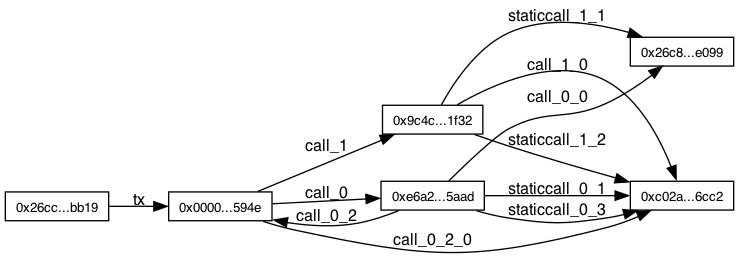
\includegraphics[width=1\textwidth]{Figures/methods/traces.png}
  \caption{Example of the structure of traces in a transaction.}
  \label{fig:traces}
\end{figure}

The only reference to the error is present in the single trace that failed, with an {\tt error} field. To understand if a deployment or the destruction successfully completed, it is necessary to propagate the error from the failed traces to all its children. Eth2dgraph does so with the algorithm reported in \cref{lst:error-propagation}. It first groups traces of a block based on transaction hash. Then, for each transaction, it gets its failed traces. Then it loops again on all the traces of the transaction to see if any of them is a child of a failed one. This is done by searching a failed trace that has a matching starting address, e.g. a trace with address {\tt 1, 0, 0} has a matching starting address of the trace {\tt 1, 0, 0, 2}.

Contract deployments and destructions found in failed traces are stored in the output of eth2dgraph with a boolean field indicating it.

\begin{lstlisting}[language=Rust,caption={Algorithm for errors propagation in traces.},label={lst:error-propagation},captionpos=b, style=boxed]
fn propagate_errors(traces: &mut Vec<Trace>) {
    // group traces by transaction hash
    let mut txs: HashMap<TxHash, Vec<&mut Trace>> = HashMap::new();
    traces.iter_mut().for_each(|t| {
        if t.transaction_hash.is_some() {
            let group = txs
                .entry(t.transaction_hash.unwrap().clone())
                .or_insert(vec![]);
            group.push(t);
        }
    });
    // inside each transaction, mark trace as failed if a parent trace has failed
    txs.iter_mut().for_each(|(_, grouped_traces)| {
        // collect trace addresses of failed traces
        let failed = grouped_traces
            .iter()
            .filter(|t| t.error.is_some())
            .map(|t| t.trace_address.clone())
            .collect::<Vec<Vec<usize>>>();
        // loop again traces to flag ones whose parent failed
        grouped_traces.iter_mut().for_each(|t| {
            let address = t.trace_address.as_slice();
            let parent_failed = failed.iter().any(|f| address.starts_with(f));
            if parent_failed {
                t.error = Some("Parent failed".to_string());
            }
        });
    });
}
\end{lstlisting}

\subsection{Accounts}

As for the smart contracts, there is no RPC to get the list of accounts used on the Ethereum blockchain. They must be extracted as they are used.

Being a permissionless blockchain implies that there is not an initial phase of registration or an official opening of an account. Users simply generate an address and start using it. 

Eth2dgraph stores accounts every time they are used in the following cases:

\begin{itemize}
    \item Senders or receivers of transactions.
    \item Receivers of validator withdrawals.
    \item Authors of blocks (miners).
    \item Receivers of SELFDESTRUCT reward.
    \item Deployer of a smart contract.
    \item Senders or receivers of token transfers.
    \item Addresses of contract deployment or destruction, marked as contracts.
    \item Addresses of contract emitting logs, marked as contracts.
    \item Addresses of a contract emitting a token transfer, marked as contract.
\end{itemize}

\section{Semantics extraction}

The previous section described how raw Ethereum data is extracted. In this section, I describe how eth2dgraph extracts semantics from this data.

The semantics extracted are meant to give a more comprehensive description of the smart contracts stored on the blockchain. The only information that can be taken from the Ethereum protocol about smart contracts is their EVM bytecode. The EVM bytecode is the byte representation of the contracts' compiled code that can be run by the Ethereum Virtual Machine implemented in all the nodes. While it is fundamental to the functioning of the protocol, it does not give any meaningful description of the smart contract for a human analysis. 

Eth2dgraph tries to put together pieces of information to allow for an easier analysis of such smart contracts.

\subsection{ABI extraction}

\label{decompilation-section}
Smart contracts are described by an \textbf{Application Binary Interface} (ABI) that lists all the functions and events that are implemented. 

Smart contracts can be seen as REST APIs. The application status is stored in the contract's private code, similar to a database.
The public functions exposed by the contract are like the API endpoints that can be used by users to interact with the application. This is done via stateless transactions (in the blockchain) and via API calls (in the traditional REST API pattern). The ABI is the description of the exposed functions, similarly to the specification of an API. 

It is clear that having the ABI of a smart contract gives many useful insights about what it does. It can also be used to decode transactions and logs. In the ABI, there are the types of functions and events arguments. These types can be used to decode the bytes present in the transactions and logs data. It is possible to understand if they represent addresses, numbers, strings, bytes, etc..

To extract the ABI, eth2dgraph integrates heimdall-rs\footnote{EVM decompiler written in Rust, source code available at: \url{https://github.com/Jon-Becker/heimdall-rs}}, an open-source EVM decompiler. Heimdall-rs uses symbolic execution to create the control flow graph (CFG) of the EVM bytecode. This is done via a custom implementation of the EVM. From the CFG, and looking at the function dispatcher part of the code, it is possible to locate functions and extract their inputs and outputs parameter types.

It is possible to extract function names using a database of reverse hashes. Function selectors are stored in the bytecode as the first four bytes of the hash of the functions' signature. It is possible to read these four bytes and see if there are matching signature that were previously reverse hashed. Heimdall-rs does this using the public etherface\footnote{Etherface is a database of Ethereum functions and event signatures, with related hashes, available at: \url{https://www.etherface.io/}} database. 
Unfortunately, it is not possible to extract parameters name from the bytecode stored on the blockchain. This piece of information is removed during the compilation of the code. 

Heimdall-rs is integrated in eth2graph using separate processes. Each time there is the need of running the decompiler, eth2dgraph creates a new process. This is done for isolation. For the nature of how the decompiler works, it can run in infinite loops during the symbolic execution. To avoid that, eth2dgraph has a parameter to set the maximum time spent waiting for de-compilation. The default is  five seconds.

The output or the heimdall-rs process is stored to text files. When decompilation is done, these files are de-serialized by eth2dgraph into Rust data structures. \cref{fig:decompilation-architecture} shows how decompilation in handled in eth2dgraph.

\begin{figure}[H]
  \centering
  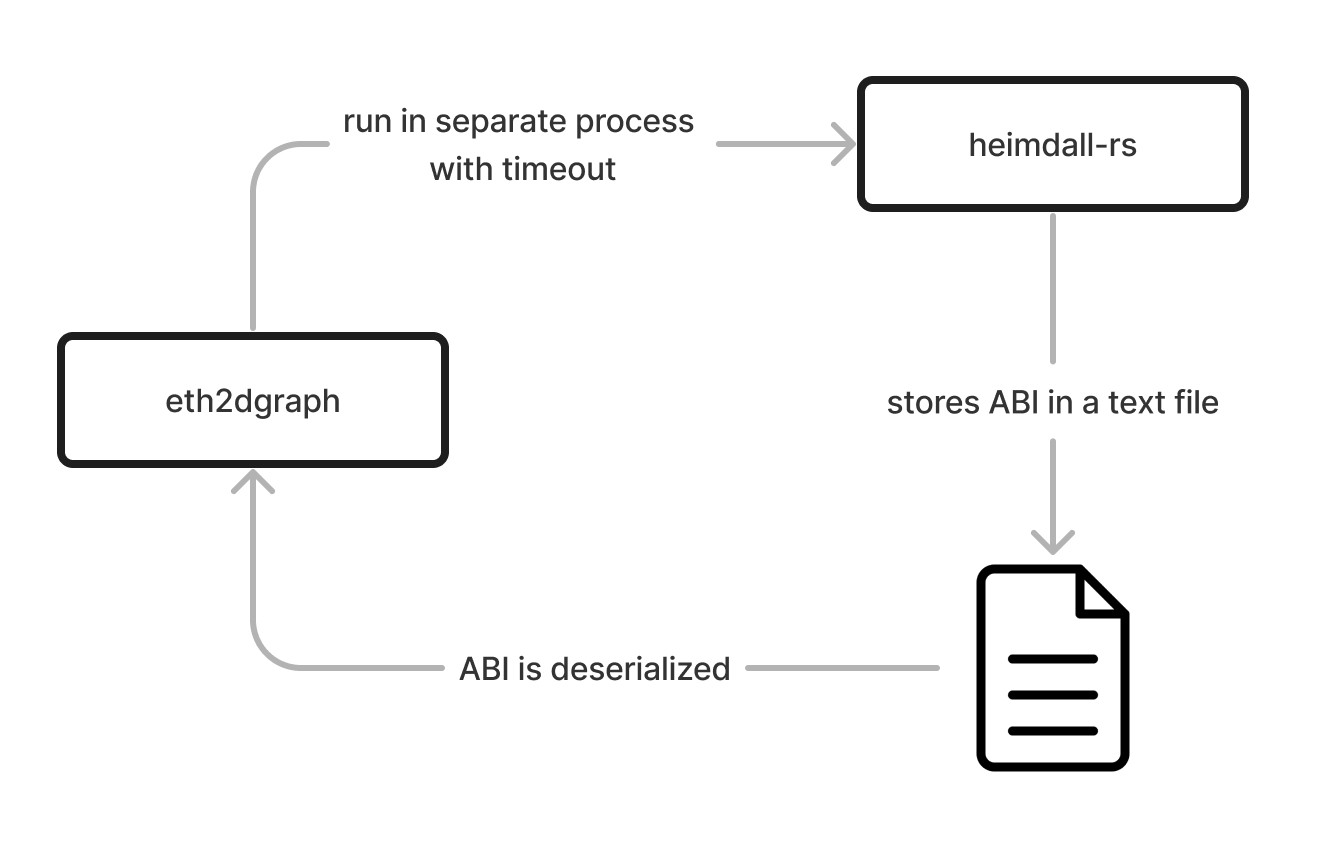
\includegraphics[width=1\textwidth]{Figures/methods/decompilation-architecture.jpg}
  \caption[Heimdall-rs integration into eth2dgraph]{Heimdall-rs integration into eth2dgraph}
  \label{fig:decompilation-architecture}
\end{figure}

\subsection{Contracts skeleton and metadata}
\label{skeleton-section}
The \textit{skeleton} of an EVM bytecode is the bytecode itself with all the arguments of the PUSH opcode set to zero. It allows to find bytecodes that are functionally identical between them. The concept of skeleton is used in many studies to reduce the total number of contracts to analyze~\cite{token-contracts}\cite{wallet-contracts}.

Removing the PUSH arguments to the bytecode deployed on the blockchain is not enough to extract the skeletons. The Solidity compiler can add metadata at the end of the bytecode that must be removed before getting the skeleton.  

Eth2dgraph identifies this part using a regular expression. Metadata is stored as CBOR\footnote{CBOR is a binary data serialization format standardized in RFC8949 \url{https://www.rfc-editor.org/rfc/rfc8949.html}} encoded data. After being splitted, the \textit{runtime} part of the bytecode is processed for the skeleton extraction, while the metadata part is decoded. Metadata are also stored in the indexed data, these are the field included:

\begin{itemize}
    \item \textit{storage\_protocol}: distributed file system protocol where the developer can eventually store the source code of the contract.
    \item \textit{storage\_hash}: location on the contract's data in the distributed file system.
    \item \textit{compiler}: the version of the Solidity compiler used.
    \item \textit{experimental}: whether the compilation was performed with experimental features activated.
\end{itemize}

The skeleton extraction is performed by looping trough the bytes of the EVM bytecode. A byte between \texttt{0x60} and \texttt{0x7f} represents a PUSH instruction. If a byte is found in that range, the next bytes are replaced with zeros depending on the kind of PUSH found. 

\subsection{Verified source code}

It is possible to link contracts to their verified source code using the repository of \textit{Smart Contract Sanctuary}~\cite{smart_contract_sanctuary}. After cloning the repository locally, eth2dgraph can be ran with an option to include source code of the discovered contracts in the indexed data.

This allows querying the contracts based on text inside the source code. Dgraph supports text matching with stemming stop words removal. Data can be queried with two query functions: \texttt{anyoftext} and \texttt{alloftext}.

\subsection{Token transfers}

The ERC20 and ERC721 token standards states that when a token ownership is transferred an event MUST be emitted. \cref{lst:erc20-transfer} shows the event emitted for fungible token transfers, \cref{lst:erc721-transfer} shows the one emitted for NFT transfers. Emitting an event means generating a log that is indexed by Ethereum nodes.

\begin{lstlisting}[caption={Event emitted for ERC20 token transfer},label={lst:erc20-transfer},captionpos=b]
event Transfer(address indexed _from, address indexed _to, uint256 _value)
\end{lstlisting}

\begin{lstlisting}[caption={Event emitted for ERC721 token transfer},label={lst:erc721-transfer},captionpos=b]
event Transfer(address indexed _from, address indexed _to, uint256 indexed _tokenId)
\end{lstlisting}

Both events share the same name and types. The only difference is in the last parameter. It is indexed in case of ERC721 and not indexed in case of ERC20. The signature of the event is not influenced by this difference, so all the logs that are describing token transfers share the same signature.

Logs with the first topic matching the keccak256 hash of the Transfer event signature are treated as token transfer by eth2dgraph.

After finding a matching log, the bytes composing the data field are split into 256 bit words and merged to the 256 words of the indexed topics.

The 256 bit words are then treated and decoded as follows:

\begin{itemize}
    \item First word is the \textit{from} address.
    \item Second word is the \textit{to} address.
    \item Third word is the \textit{value}. It represent the amount in case of ERC20 or the token ID in case of ERC721.
\end{itemize}

If the decoding succeeds, the log is parsed and later stored as a token transfer.

Distinction between ERC20 and ERC721 transfers is done based on length of the topics array. Since ERC20 has the last parameter not indexed, the topics length is three words. For the ERC721 the topics length is four. This information is used to discriminate between storing the third word as \textit{value} or as \textit{token\_id}.

The same way of semantics extraction can be used for other kind of logs, e.g. token swaps. Eth2dgraph implements the code for parsing token transfer since it is the most common log emitted on the Ethereum chain.

\section{Software architecture}

The Ethereum network stores data in the order of billions of entries. The process of extraction must be as efficient as possible to be able to get this data in reasonable time. At the time of writing, Ethereum has 17.5M blocks. Performing each single action described in the previous sections sequentially for each block results in executions that take many days or even weeks. 

A lot of time is spent waiting for network data (the calls to the RPCs) or for the decompiler process to complete the decompilation. While it is not possible to make these steps faster, it is possible to parallelize them. Eth2dgraph has been developed to maximize concurrency of the machine where it is ran to minimize the time needed for data extraction.

This was done using async Rust and the \textit{Tokio asyncronous runtime}\footnote{Tokio provides a multi-threaded runtime for executing asynchronous Rust code \url{https://tokio.rs/}.}. \cref{fig:eth2dgraph-architecture} gives a general overview of how tasks are used and how they communicate.

\begin{figure}[H]
  \centering
  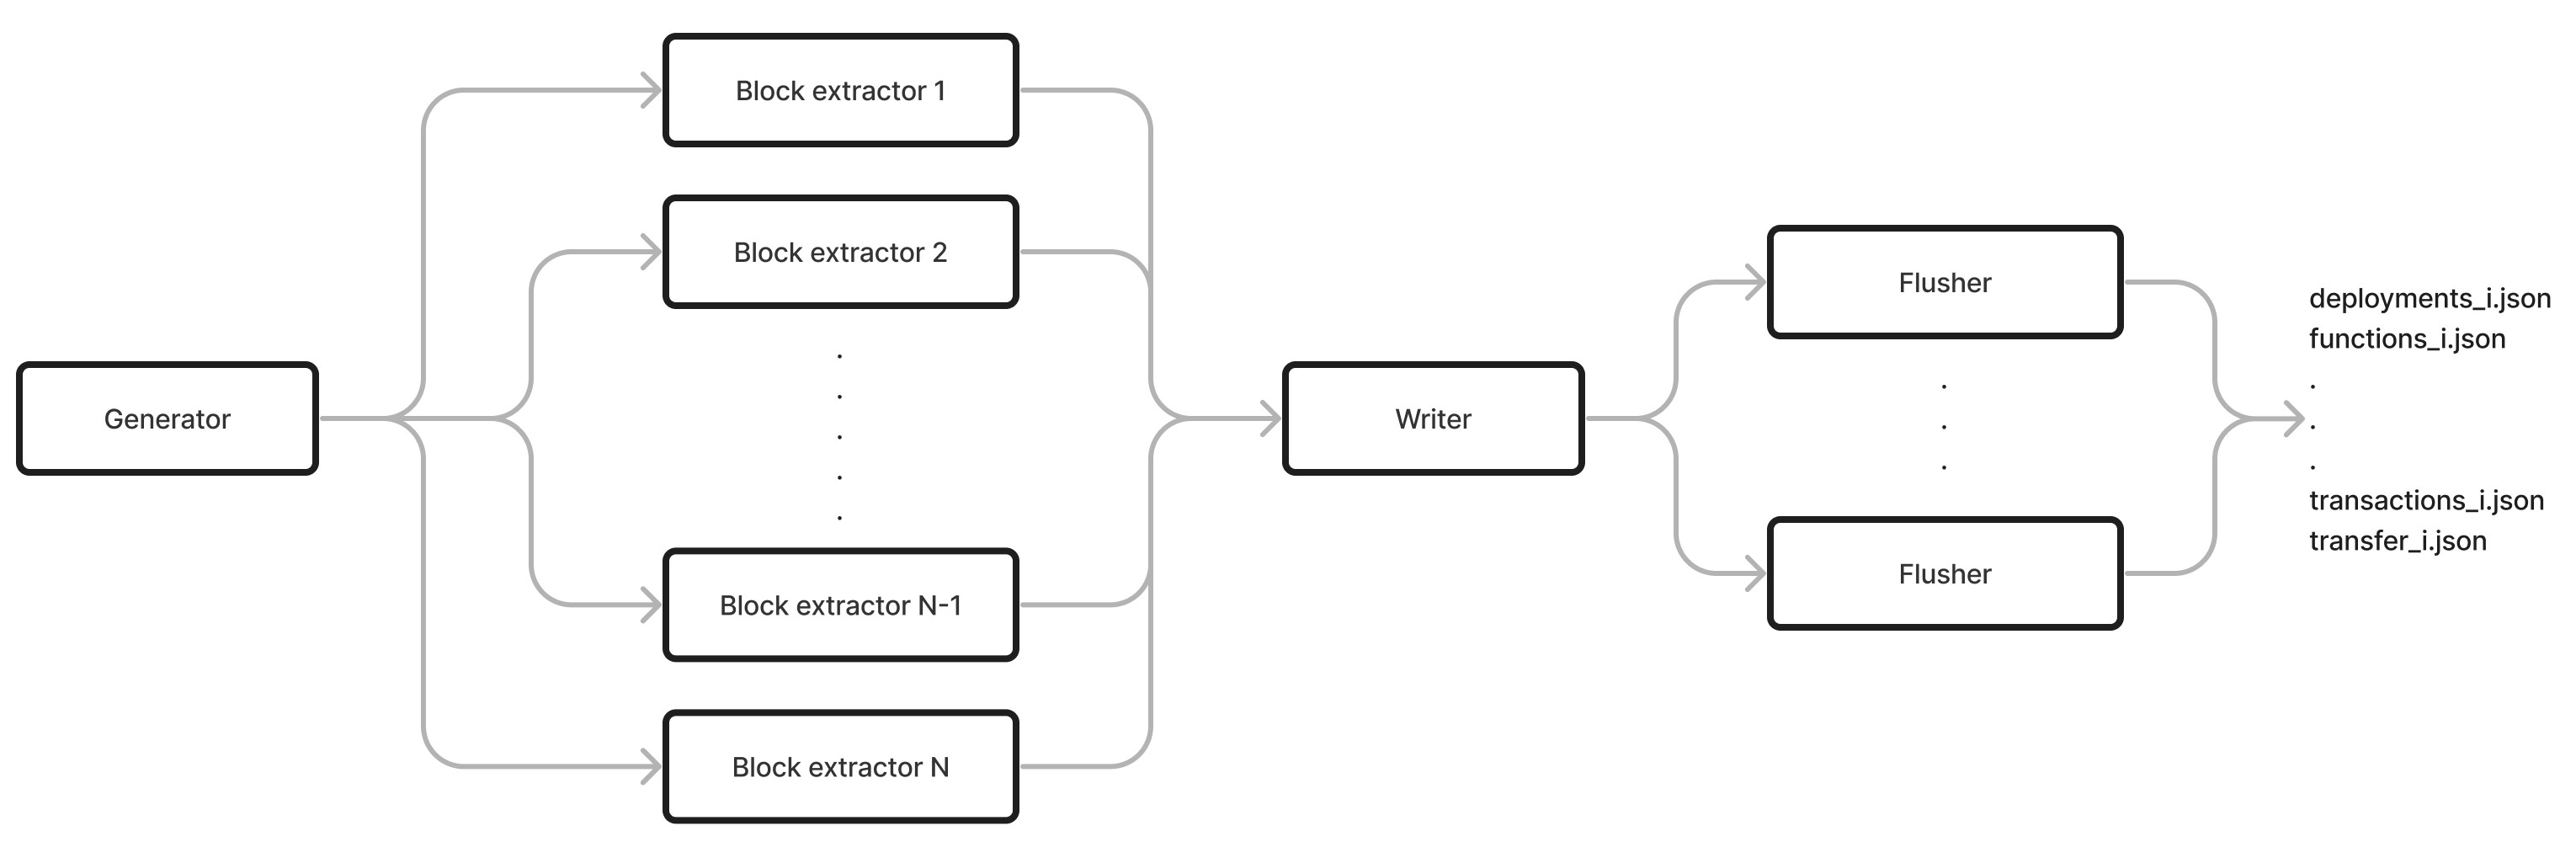
\includegraphics[width=1\textwidth]{Figures/methods/software-architecture.jpg}
  \caption[Software architecture of eth2dgraph]{Software architecture of eth2dgraph}
  \label{fig:eth2dgraph-architecture}
\end{figure}

Here is a more detailed description of each task:

\begin{itemize}
    \item The \textit{generator} task loops trough the block range to extract and spawns, using \texttt{tokio::spawn}, an \textit{extractor} task for each block that must be processed. It is also responsible for initializing all the data structures needed, the output data folders and the \textit{writer} task. 
    
    It is possible to set the limit of parallel extractor tasks to run usign the \texttt{--num-jobs} option. This is implemented using a semaphore. Each time an extractor task is created, it acquires a permit from a semaphore with a fixed capacity. When the task ends, the permit is dropped and, as a consequence, a new permit is freed in the semaphore. In case the maximum number of tasks is reached, the generator waits until the semaphore has a free permit available. This was done to avoid overloading the system with millions of concurrent tasks.

    \item The extractor task is the one responsible for the actual extraction. It receive as an argument the block to process and it collects all the data related to it. This includes handling the decompilation. All the steps related to data extraction were described in the previous sections.

    When data is ready to be stored, it is sent to the writer task using a bounded \textit{multiple-producer single-consumer} (mpsc) channel.

    \item The writer task is responsible to collect all the data sent by all the extractors and merge it. It stores data in buffers, one for each data type. When buffers reach a certain size, that can be set with the \texttt{--size-output} option, they are sent to a \textit{flusher} task to be stored to disk. The flusher tasks are spawned on demand by the writer task using \texttt{tokio::spawn\_blocking}. All their join handles are stored in a vector to wait for their termination at the end of the extraction.

    \item The flusher task is responsible for storing and compressing the output of the extraction. It receives a vector of a generic type \texttt{T} that implements the trait \texttt{SerializeDgraph}. It compresses this vector using gzip with a compression level that can be set as an option. Finally, it stores it in an output file. Data is stored divided by type and with incremental file names.
\end{itemize}

All these tasks are ran on the multi-threaded Tokio runtime. They are managed by the Tokio scheduler that implements a \textit{non-preemptive}, also called \textit{cooperative}, scheduling strategy. This means that tasks are switched when they explicitly ask for it, giving back the control to the scheduler. 

In this way it is possible to maximize the parallelism of the extraction process. For example, when a task is downloading block's data, it calls \texttt{await} on the library function responsible for networking. This call tells the Tokio scheduler that the task is paused and cannot continue, so it is replaced with another task that has work to do.

\subsection{Decompilation cache}
\label{cachine-section}
One of the biggest bottlenecks of the extraction process was the decompilation step. Spawning a dedicated process for handling decompilation of each contract deployment takes a lot of time. The main problem is that the decompiler, for how it is designed, can encounter infinite loops during the building of the control flow graph. To avoid that, it is ran with a timeout of a few seconds, but even with that, it was slowing down the process by a lot.

The solution implemented in eth2dgraph is caching the decompilation based on bytecode skeletons. Two contract deployments sharing the same EVM skeleton are decompiled only once. The decompiled ABI of a skeleton comes from the decompilation of the first contract found with that skeleton.

The reason of this choice is that contracts sharing the same skeleton also share the same code logic. In theory, there could be a difference in the function names, since they are stored as arguments of PUSH instructions, but, from the data analyzed, this almost never happens.

To test the reliability of the caching logic, I compared ABIs extracted from decompiling each single contract to the ones got using the cache. To make the test more reliable, I ran it on various block ranges spanning trough the history of the Ethereum blockchain. \cref{table:caching-precision} reports the results of the tests. Full match means that the ABI got from the cache is exactly the same as the one got from a new decompilation run. Partial match indicates that the ABI got from the cache has the same exact function and event names, but there is at least one difference between types based on assumptions made by the decompiler (e.g. bytes instead of address). Mismatch indicates that the ABI got from the cache has at least one different function or event name.

\begin{table}[ht!]
\centering
    \begin{threeparttable}
    \begin{tabular}{m{3cm} m{2cm} m{2cm} m{2cm} m{2.5cm}} 
    \toprule
    \textbf{Blocks range} & \textbf{Cache hits} & \textbf{Full matches} & \textbf{Partial matches} & \textbf{Mismatches}   \\
    \midrule
    6000000-6001000   & 1373 & 1373 & 0 & 0 \\
    10000000-10001000 & 596 & 592 & 4 & 0 \\
    12008000-12009000 & 1296 & 1295 & 1 & 0 \\
    15505000-15506000 & 101 & 101 & 0 & 0 \\
    16001000-16002000 & 120 & 100 & 19 & 1 \\
    17000000-17001000 & 39 & 39 & 0 & 0 \\
    \bottomrule
    \end{tabular}
    \end{threeparttable}
    \caption{Precision of the decompilation caching logic}
    \label{table:caching-precision}
\end{table}

In total, 99.29\% of the cache hits resulted in full matches, 0.68\% in partial matches and just 0.03\% in mismatches.

This level of accuracy showed that caching decompilation based on skeletons is an effective way of reducing the time needed for semantics extraction. The slight loss of precision is justified by the boost in performance, that made it possible to scale the extraction of ABIs to all the history of the chain in a single machine. It allowed to reduce the number of decompilation runs from 60M to 470k.

The cache is implemented in the code with a shared \texttt{HashMap}. The implementation of the concurrent hashmap used is the one provided by the {\tt DashMap}\footnote{DashMap provides a concurrent hashmap that is faster and easier to use that the combination of {\tt RwLock} and {\tt HashMap}. It is available at:\url{https://github.com/xacrimon/dashmap}} crate. The \textit{key} of the hashmap is the hash of the skeleton's bytecode and the \textit{value} is an \textit{atomic unsigned integer}. The role of the number in the cache is of indicating how many failures that specific skeleton has encountered during decompilation. It is used for trying multiple times to decompile a skeleton that fails to decompile even with different contracts' bytecodes. These is an hard limit of ten attempts, after which the skeleton is stored without the ABI and no more decompilation processes will be spawned.

This way of extracting semantics has a direct implication on the schema of data. The ABI extracted by the decompiler is linked to the skeleton and not to the contract deployment itself. \cref{fig:contracts-storage} shows the result of this design choice in the schema.

\begin{figure}[H]
  \centering
  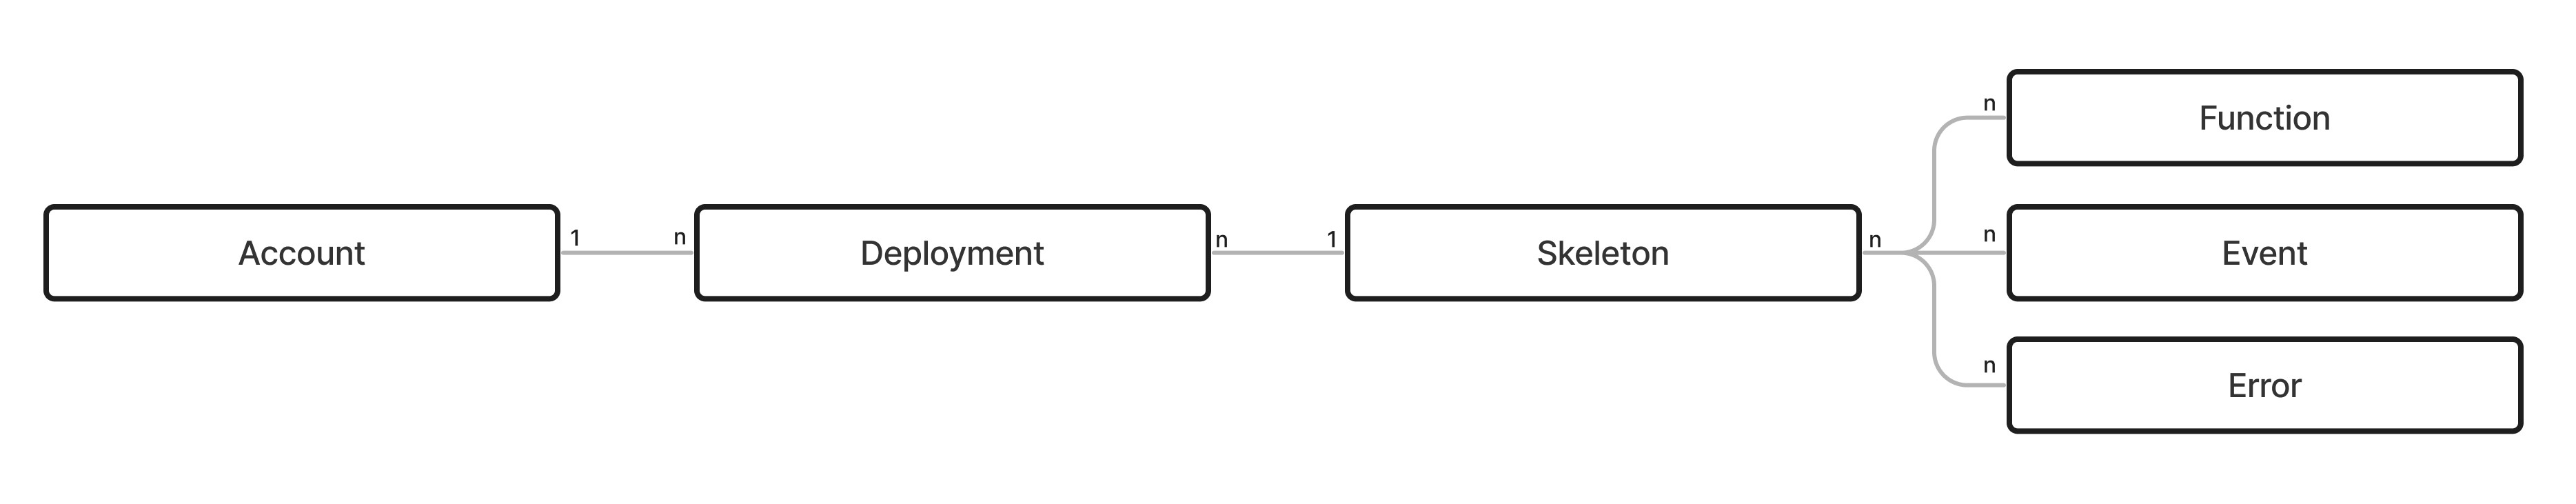
\includegraphics[width=1\textwidth]{Figures/methods/contracts-storage.jpg}
  \caption[Storage of contracts' information]{Storage of contracts' information}
  \label{fig:contracts-storage}
\end{figure}

\section{Similarity calculation}
\label{similarity-calculation}
Smart contracts' deployments are clustered based on bytecode skeletons: many smart contracts share the same skeleton and thus they are linked to the same skeleton's entity in the database. To link these skeleton clusters together, some similarity metrics are needed. Linking skeleton clusters helps the process of data analysis; it ease the recognition of patterns and connections.

Eth2dgraph implements two similarity metrics:

\begin{itemize}
    \item \textit{Interface similarity}: inspired by Di Angelo and Salzer \cite{clustering-sc}, it calculates similarity between skeletons as the Jaccard index of the sets of function and event names. Two skeletons are similar if they have similar ABIs. It is calculated as 
    \begin{equation}
	Sim = \frac{|A\cap B|}{|A\cup B|}
    \end{equation}
    where $A$ and $B$ are the sets containing function and event names. It gives a number between $1$ (identical ABIs) and $0$ (non-overlapping ABIs).
    
    \item \textit{Bytecode similarity}: The interface similarity logic works greatly if the smart contracts implement many public functions, but it doesn’t work very well if most of the code lies in internal functions and the exposed ones are just a few, like \texttt{start()} or \texttt{run()}. 
    To face this problem I added a second similarity metric that just considers the contracts' bytecodes. Inspired by Kiffer et al.~\cite{ethereum-sc-topology}, the metric used is the cosine similarity between hypervectors containing the frequencies of opcodes' 5-grams. It is computed as follows:
    \begin{enumerate}
        \item The two bytecodes to analyze are decoded to extract the opcodes, without their arguments.
        \item From the opcodes, the 5-grams and their frequencies are calculated. For example these instructions: 
        \begin{lstlisting}
PUSH1
PUSH1
MSTORE
CALLVALUE
DUP1
ISZERO
PUSH2
JUMPI
PUSH1\end{lstlisting}
        give these 5-grams with related frequencies:
        \begin{lstlisting}
[
    ("PUSH1 PUSH1 MSTORE CALLVALUE DUP1", 1),
    ("PUSH1 MSTORE CALLVALUE DUP1 ISZERO", 1),
    ("MSTORE CALLVALUE DUP1 ISZERO PUSH2", 1),
    ("CALLVALUE DUP1 ISZERO PUSH2 JUMPI", 1),
    ("DUP1 ISZERO PUSH2 JUMPI PUSH1", 1),
]       \end{lstlisting}
        \item This results in having two hypervectors, here called $A$ and $B$, in the dimension of the 5-grams. The cosine similarity is the cosine of the angle between these two vectors. It is possible to compute it as 
        \[
        cos(\theta)=\frac{A \cdot B}{||A||\,||B||}=\frac{\sum\limits_{i=1}^{n}A_iB_i}{ \sqrt{\sum\limits_{i=1}^{n}A^2_i \cdot \sum\limits_{i=1}^{n}B^2_i} }
        \]
        This gives a number between 0 (completely dissimilar bytecodes) and 1 (identical bytecodes). The suggested threshold for considering similarity suggested by Kiffer et al. is of $0.90$.
    \end{enumerate}
\end{itemize}

The process of similarity calculation is done on demand after data is loaded into Dgraph. The same binary that is responsible for the data extraction part also integrates commands to perform data analysis. 

It is possible to run eth2dgraph with the \texttt{analyse similarity} command to calculate both the previous metrics. Comparing all skeletons with each other is a heavy calculation, with a quadratic complexity with respect to the number of skeletons. It is possible to restrict the calculation to a single skeleton, giving as an argument the address of a contract.

To optimize the performances, calculation of similarity is done in parallel using the \textit{parallel iterators} of the \textit{Rayon}\footnote{Rayon is a data-parallelism library that easily introduces parallelism into existing sequential code  \url{https://docs.rs/rayon/latest/rayon/}} crate.

The output of the calculation is a text file containing the RDF triples that describe the similarities. It is possible to import it into the live database by running a mutation or using the Dgraph's \textit{live loader}.

Similarity values are stored as edge attributes, called \textit{facets} in Dgraph. It is possible to query the data filtering by similarity value. \cref{lst:skeleton-similarity-query} shows an example of how to retrieve similar skeletons filtering by similarity value.

\begin{lstlisting}[caption={Example DQL query for getting similar skeletons.},label={lst:skeleton-similarity-query},captionpos=b]
{
    q(func: uid(0x180c753f6)) {
        Skeleton.similar_code @facets(gt(similarity, 0.95)) @facets(similarity) {
            uid
        }
        Skeleton.similar_interface @facets(gt(similarity, 0.95)) @facets(similarity) {
            uid
        }
    }
}
\end{lstlisting}
\cleardoublepage


\chapter{Results}

\section{More figures}

This section includes some examples of different types of figures to include. A simple single figure is shown in figure \ref{fig:trajectory_angle}, while figure \ref{fig:cyclic} shows how three subfigures can be included together. Remember to change both the caption and the title in the square brackets before the caption, which will show up in the list of figures. \\

\noindent page fill page fill page fill page fill page fill page fill page fill page fill page fill page fill page fill page fill page fill page fill page fill page fill page fill page fill page fill page fill page fill page fill page fill page fill page fill page fill page fill page fill page fill page fill page fill page fill page fill page fill page fill page fill page fill page fill page fill page fill page fill page fill page fill page fill page fill page fill.

\begin{figure}[H]
  \centering
  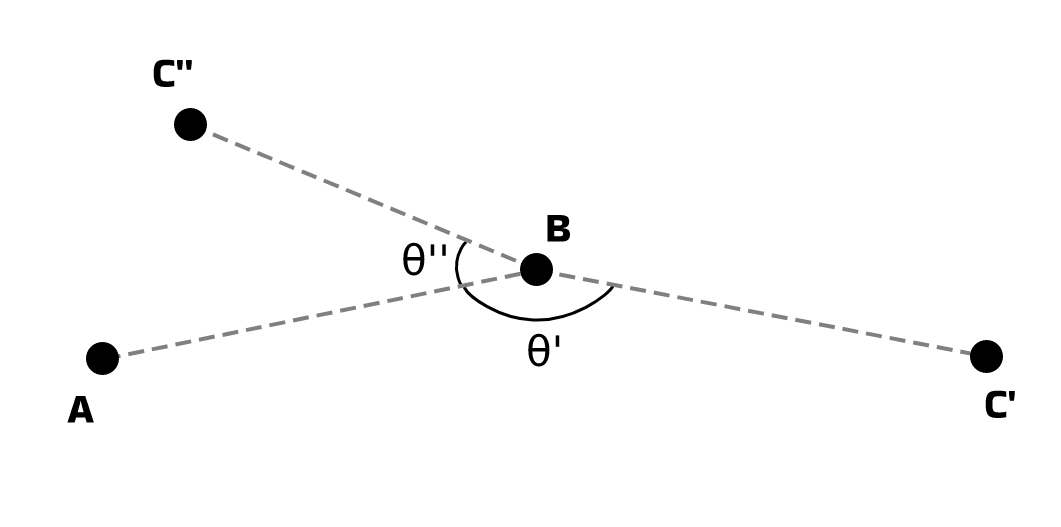
\includegraphics[width=1\textwidth]{Figures/trajectory angle.png}
  \caption[Trajectory angle]{The trajectory angle found for the trajectory ABC between the three points A, B and C. The two different C-points show the angle gotten for relatively unchanged directional trajectory with C', and opposite directional trajectory with C''.}
  \label{fig:trajectory_angle}
\end{figure}



\begin{figure}[H]
  \centering
  \subfloat[Time as a linear variable.]{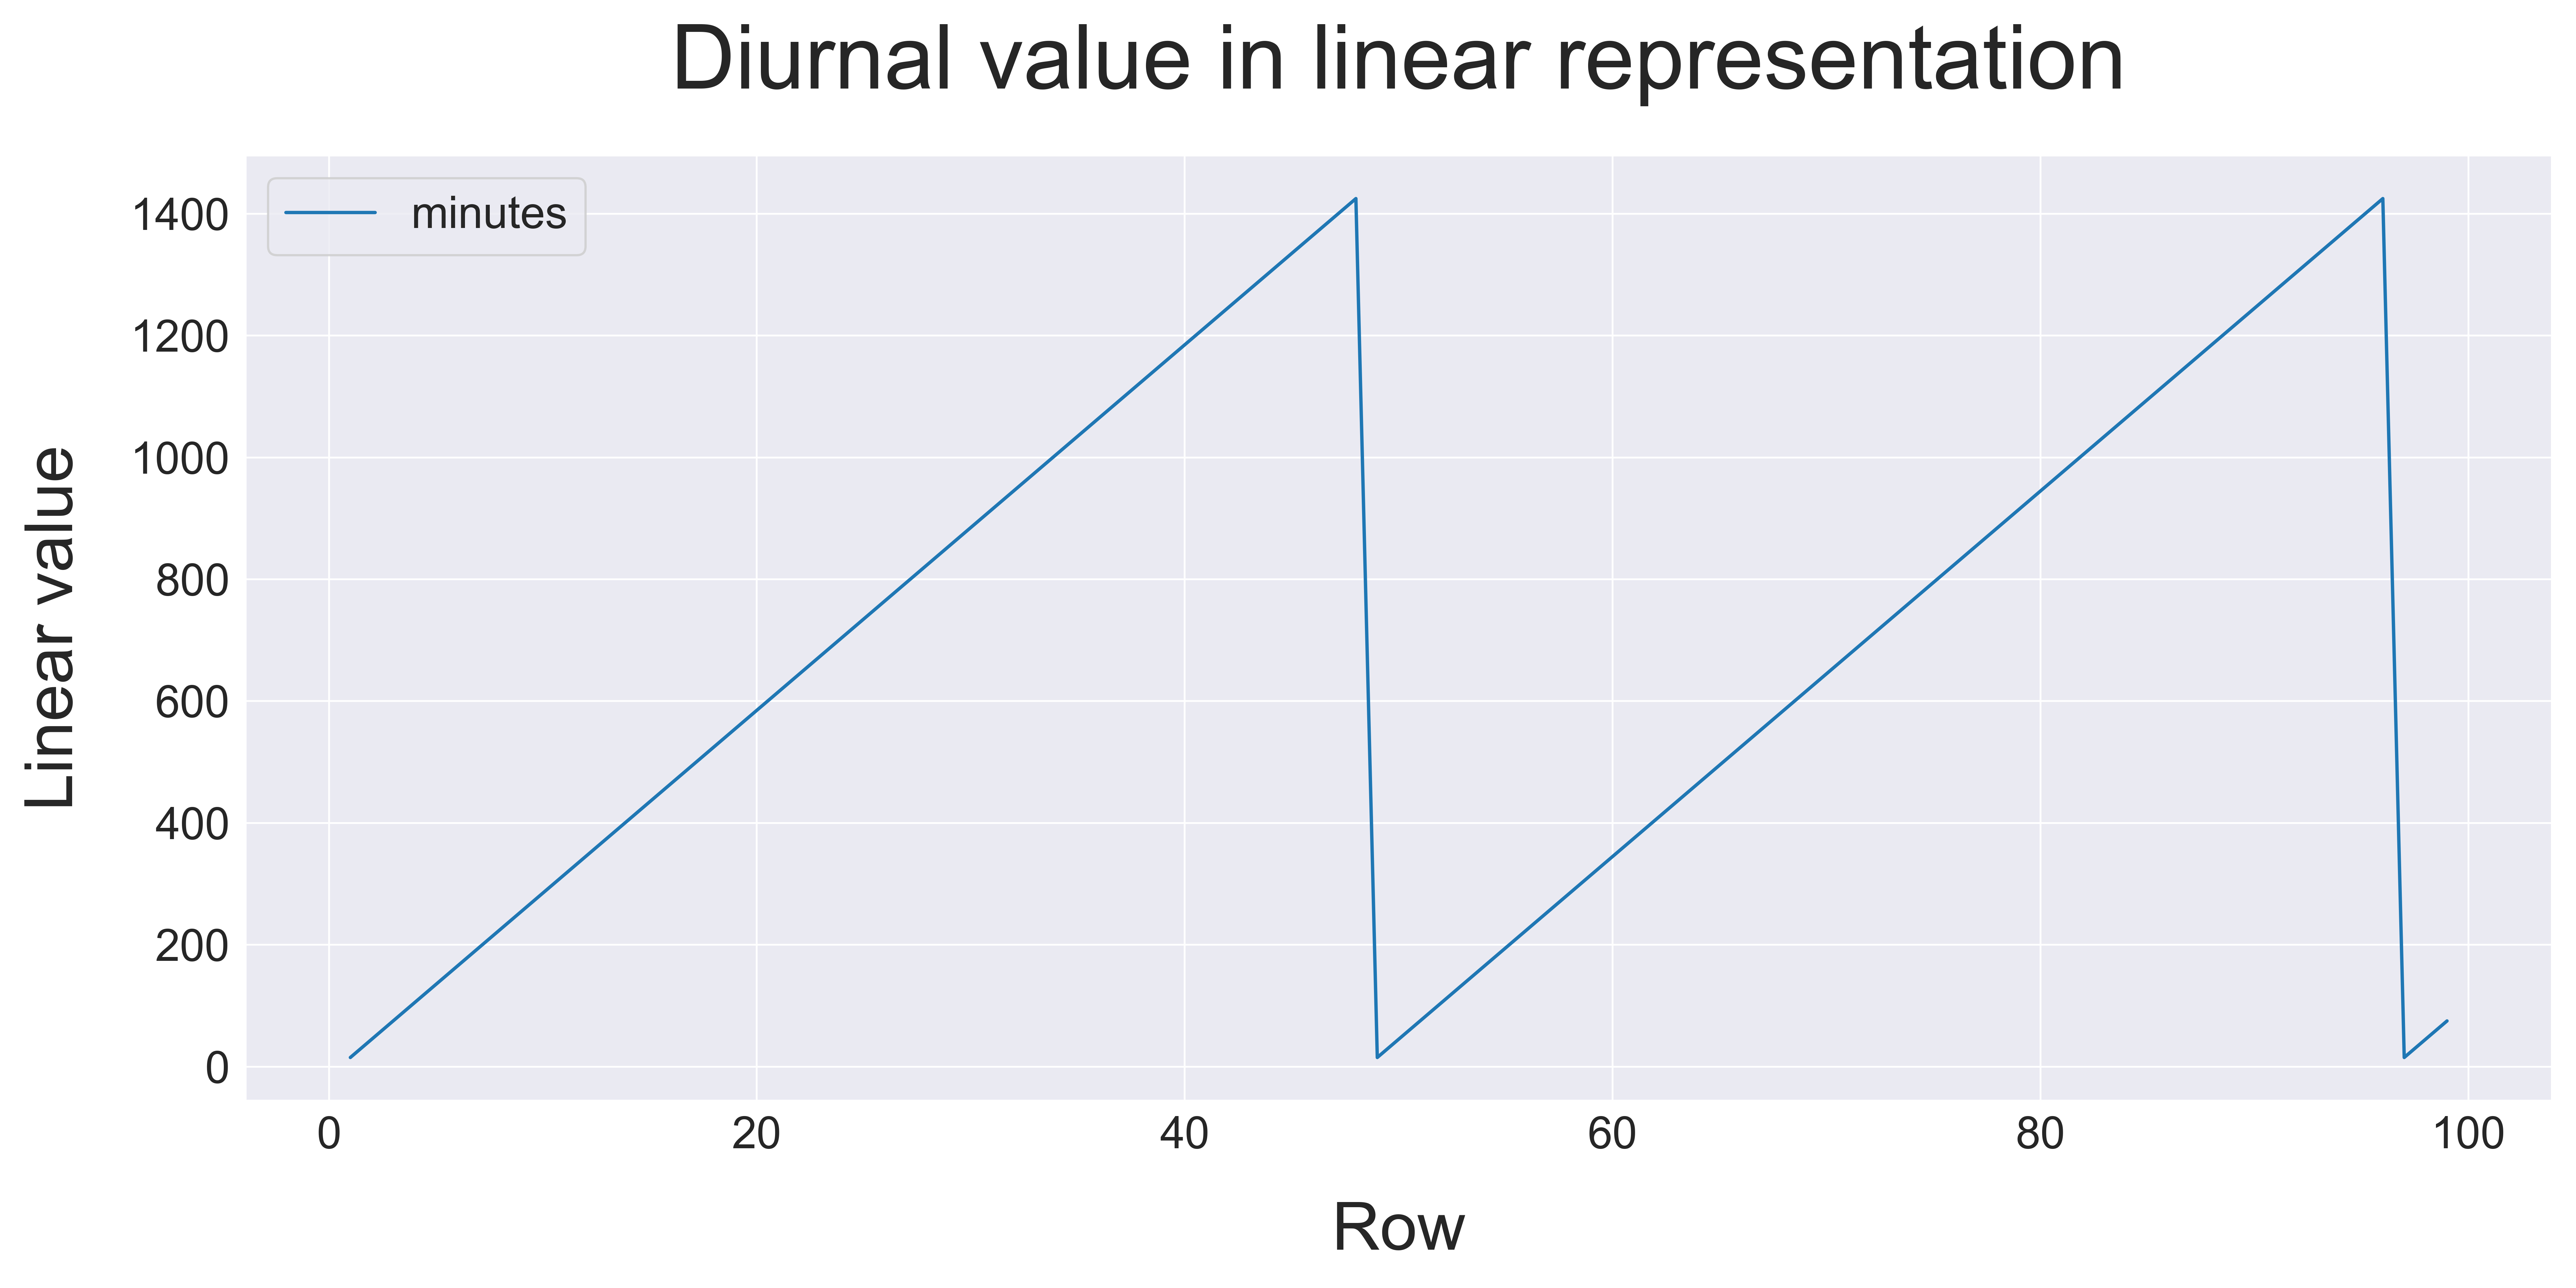
\includegraphics[width=0.75\textwidth]{Figures/diurnal_values_linear.png}\label{fig:diurnal_lin}}
  \hfill
  \subfloat[Time represented as pairs of sine and cosine.]{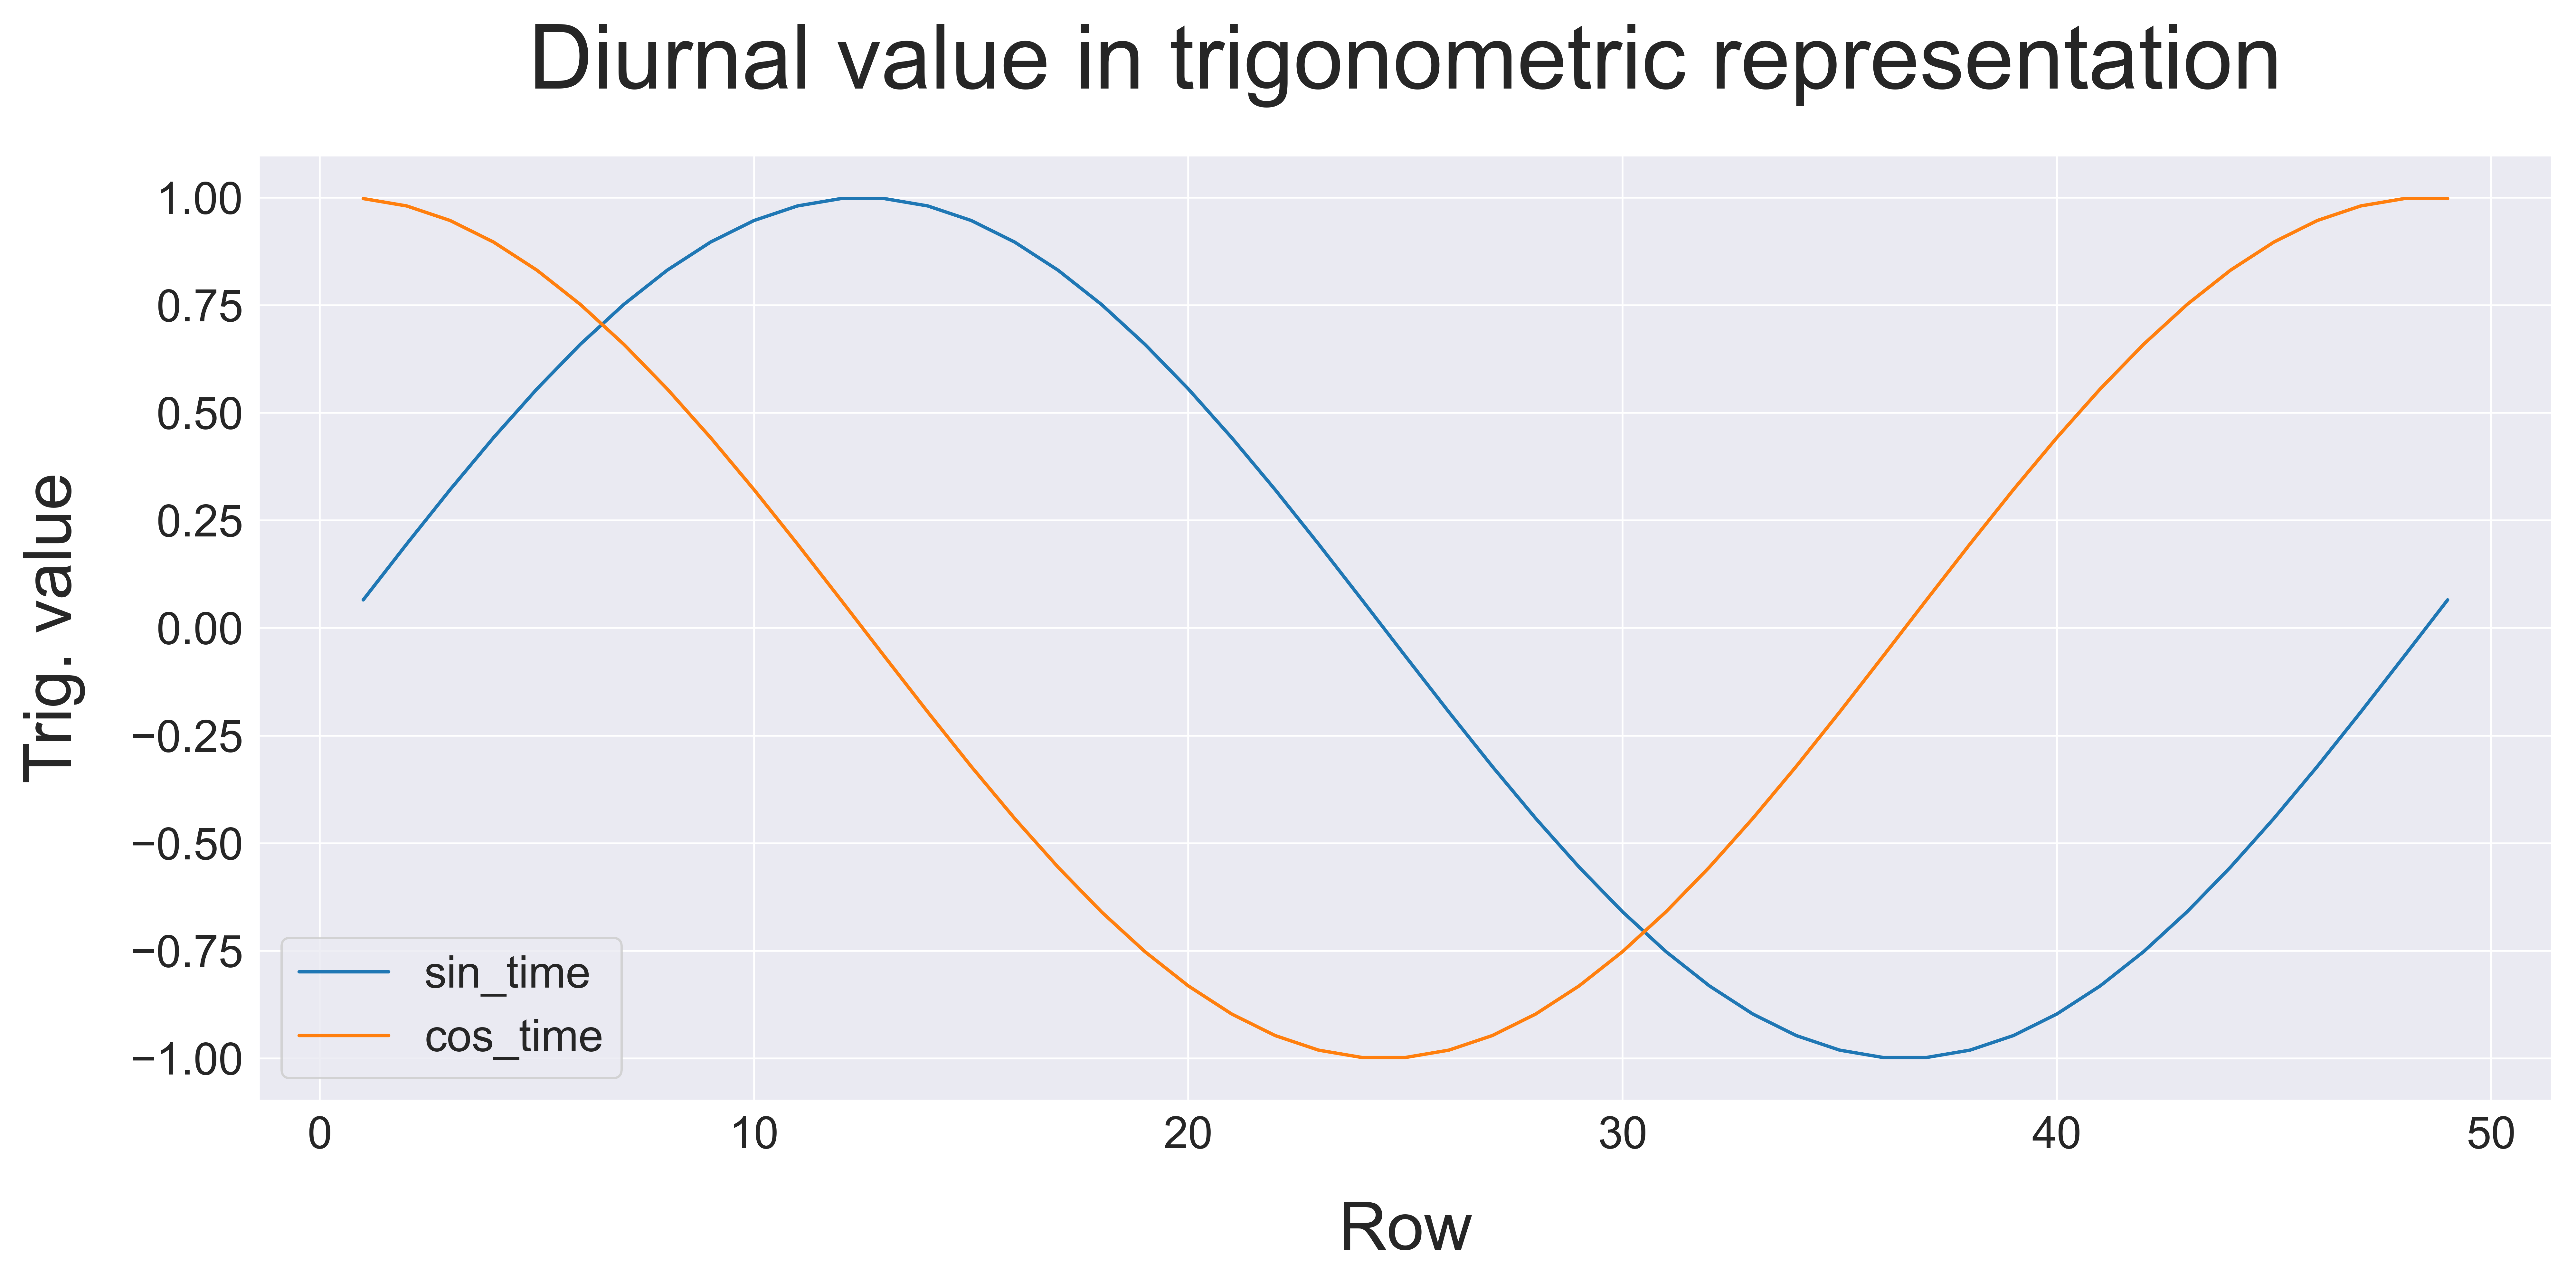
\includegraphics[width=0.75\textwidth]{Figures/diurnal_values_sine.png}\label{fig:diurnal_trig}}
  \hfill
  \subfloat[Time as a cyclic feature.]{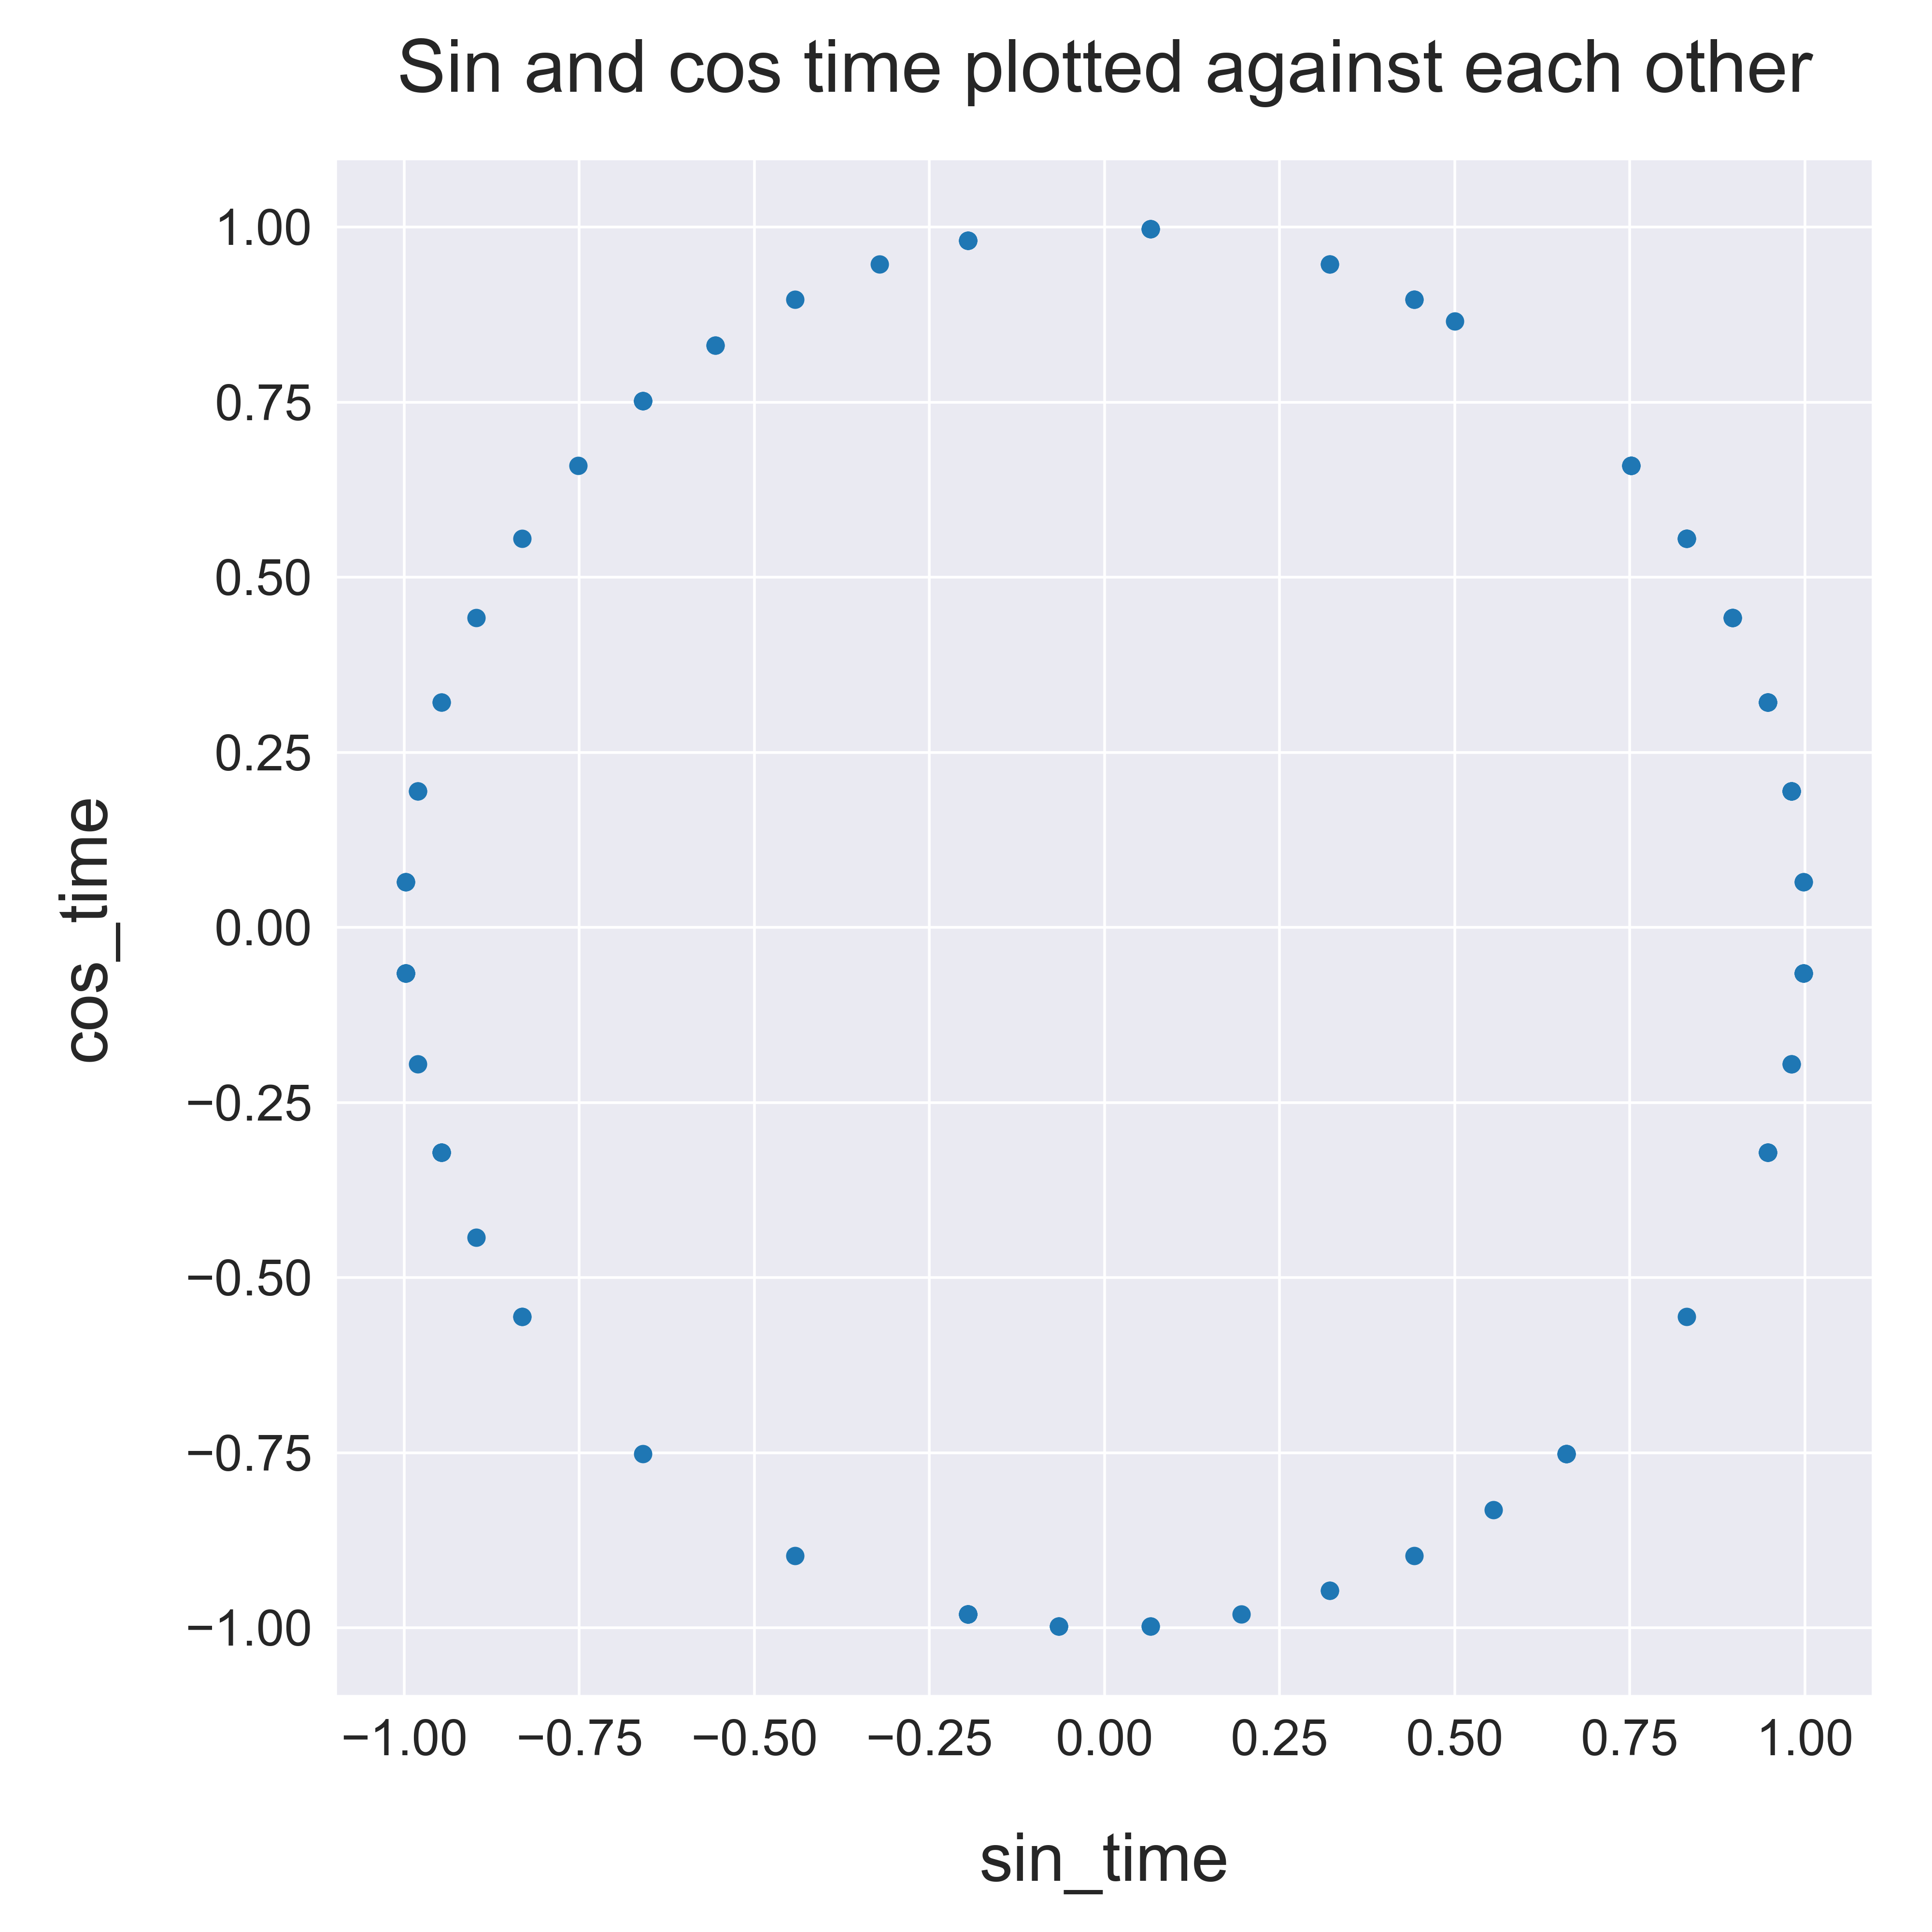
\includegraphics[width=0.6\textwidth]{Figures/diurnal_values_circle.png}\label{fig:diurnal_cyclic}}
  
  \caption[Time as a cyclic feature]{Figure (a) shows the time variable in the data for the first 100 rows using linear time as minutes past midnight, figure (b) shows the trigonometric time representation for one cycle where each time point has a unique sine and cosine-pair value, and figure (c) shows time as a cyclic feature with the trigonometric pairs.}
\label{fig:cyclic}
\end{figure}
\cleardoublepage


\chapter{Discussion}

Discuss your results here.

\section{Future work}

Include a section about what should or could be done in future research, or explain any recommended next steps based on the results you got. This should be the last section in the discussion.
\cleardoublepage


\chapter{Conclusions}
\label{chapter-7}


\cleardoublepage


\addcontentsline{toc}{chapter}{\protect\numberline{}References}
\printbibliography[title={References}] %you may change the title in the toc here if you want
\cleardoublepage


\chapter*{\LARGE \textbf{Appendices}}
\fancyhf{} %clear the header, it should be empty for the appendices
\renewcommand{\headrulewidth}{0pt} %no rule
\fancyfoot[C]{\thepage} %set the page numbers in the center of the footer instead 

%it is possible to set a different page numbering style for the appendix, but I personally just continued with the same page numbering as the main content as I find that more tidy
%\pagenumbering{roman}
%\setcounter{page}{1}
\addcontentsline{toc}{chapter}{\protect\numberline{}Appendices:}
\appendix


\chapter*{A - Github repository}
\addcontentsline{toc}{chapter}{\protect\numberline{}A - Github repository} 

All code and latex-files used in this document are included in the Github repository linked below. Further explanations are given in the readme-file. 


\subsection*{Github repository link}
\begin{itemize}
    \item \url{https://github.com/ninasalvesen/thesis_latex_template}
\end{itemize}


\end{document}
